% !TEX root = ../report_kenko.tex

%---------------------------------------------------------------------------
\chapter{健康寿命の事業の概要}
%---------------------------------------------------------------------------
\section{背景}
日本は, ここ25年の間, 平均寿命の延伸, 死亡率の低下により, 高齢化率が2016年において27\%を示しており, 既に「高齢社会(総人口に対して65歳以上の割合が14\%以上)」を過ぎて「超高齢社会」に入っている.\footnote{
	高齢化率とは総人口に対して65歳以上の高齢者人口が占める割合. 世界保健機構(WHO)や国連の定義によると, 高齢化率が7%を超えた社会を「高齢化社会」, 14%を超えた社会を「高齢社会」, 21%を超えた社会を「超高齢社会」と定義.
}
また, 野村ら(Lancet, 2017)の研究では, 「疾病の地域格差(regional variation of disease)」問題を指摘し, 国の保健政策への反映を求めている. こうした結果は, 国・自治体が, 限らた健康予算の配分の中で 「健康の質の向上」政策に転化する必要があることを意味する. 海外では既に国の保健対策をデータに基づいて行う変革が実施されており, この事例は滋賀県の保健活動にも示唆に富んでいる(Global Burden of Disease :  Generating Evidence, Guiding Policy, 2010).
\section{目的}
健康の質を表す健康寿命やそれと関連のある指標を用いて統計解析し, 滋賀県の位置づけや強み・弱みを把握し, 今後, 滋賀県の健康政策立案に役に立つ根拠を示すことを目的とする.
\section{実施期間}
平成29年8月25日$\sim$平成30年3月31日まで

\section{データ}
滋賀県衛生科学センターの既調査データ, 保健と関連のある公表データ, 既発表の研究データなどを利用する.

\section{方法}
都道府県間の健康指標の比較を行った野村ら(Lancet, 2017)の研究の方法論を参考にしながら, より滋賀県の視点から滋賀県を中心として統計分析を実施する. 上記の「データ」を用いて, 解析には主に統計ソフトRを利用する. 提供データの形式に最も適合する最新の可視化統計手法を取り入れ, 探索データ解析を行うとともに, 健康寿命に影響を与える要因を探るため,  医学的変数のほか, 社会的説明変数を絞り込み, 多変量解析, 一般化線形モデリング解析などを行う. なお, 解析の方針と統計手法の詳細は, 担当者の間で意見交換しあい, 適切な方法を取り入れる.


\section{期待効果}
県民向けには本県が「住みやすい街」,「健康な県」という事実を再認識され, 県外在住者には移住促進政策のための発信情報として活用できると期待される.
ビックデータ時代に, 他県に先駆けて官学連携による健康データを活用する取り組みは, データに基づく県政を推奨している国の方針とも当てはまるので, 他県のベンチマーク事例になることが期待される.

%------------------------------------------------------------
\chapter{なぜ滋賀県が健康・長寿県となれたのか}
%------------------------------------------------------------
滋賀県は2000年には健康, 寿命に関する調査で中位に留まっていたが,
2013年の調査では躍進した結果となった.
野村ら(Lancet, 2017)を含め最近の報告では, 滋賀県は健康に関する様々な指標において上位に位置している.
その理由を理解するためには, これまで滋賀県が取り組んで来た保健対策や組織の変遷について, 時系列的に
どのような変化があったのか調べる必要がある.

%————————————————————
\section{組織体制}
%————————————————————
\subsection{健康推進連絡協議(1987〜, 民間)}
%————————————————————
滋賀県の「健康推進連絡協議会」は1987年度に, 母子保健推進員と食生活改善推進員が合体し, 地域において歯科保健も含めたさまざまな分野の健康活動を行っている.
\begin{itemize} \setlength{\itemsep}{-0.5mm} \setlength{\parskip}{-0.5mm}

	\item  ボランティア組織
	\item  市町に地域での健康づくり活動
	      \begin{itemize} \setlength{\itemsep}{-0.5mm} \setlength{\parskip}{-0.5mm}
		      \item 2016年度総人数 3,612人
	      \end{itemize}
	\item  毎年養成研修会を実施
	      \begin{itemize} \setlength{\itemsep}{-0.5mm} \setlength{\parskip}{-0.5mm}
		      \item 2016年, 養成講座受講実績, 407人
	      \end{itemize}
\end{itemize}

%————————————————————
\subsection{健康づくり県民会議(1994〜2010)}
%————————————————————
\begin{itemize} \setlength{\itemsep}{-0.5mm} \setlength{\parskip}{-0.5mm}
	\item 5分野(栄養, 運動, 休養, 健診, 生きがい)で構成
	      \begin{itemize} \setlength{\itemsep}{-0.5mm} \setlength{\parskip}{-0.5mm}
		      \item それぞれ10名, 計50名からなる組織
	      \end{itemize}
	\item 活動内容 : 県民運動としての健康づくり
	\item 成果 : 「健康づくりガイドブック」を県内全戸配布
\end{itemize}
2010年以降, 「健康づくり県民会議」は, 予算削減に伴って, 活動は停止状態となっている.

%————————————————————
\subsection{健康づくり支援室(2001〜2009)}
%————————————————————
1999年度, 国において「健康日本21」が策定された.\footnote{「健康日本21」とは
	%1999年度策定された
	「国民の健康の増進の目標」を定めたのも. 2012年に全部改正(厚生労働省告示430号)し現在は「健康日本(第2次)」.}
これを受けて滋賀県は,
\begin{itemize} \setlength{\itemsep}{-0.5mm} \setlength{\parskip}{-0.5mm}
	\item 2000年度には, 県の健康増進計画である「健康いきいき21健康滋賀推進プラン」が策定
	\item 2001年〜2009年度の間「健康づくり支援室」を運営
\end{itemize}
など国の健康政策に協力的かつ迅速に対応した.

健康増進計画策定に当たって, 「健康づくり支援室」の主な活動と成果は
\begin{itemize} \setlength{\itemsep}{-0.5mm} \setlength{\parskip}{-0.5mm}
	\item 「健康づくり支援資料集」を作成
	      \begin{itemize} \setlength{\itemsep}{-0.5mm} \setlength{\parskip}{-0.5mm}
		      \item 人口動態統計, 医療費情報, 計画目標11分野関連情報等, 健康関連の情報をオールインワンでまとめたもの
	      \end{itemize}
	\item 保健所, 市町等関連組織に配布
	\item この資料集を活用しながら, 県, 市町が科学的根拠に基づいた保健活動の推進, 客観的評価に基づいたP-D-C-Aサイクルの実施
\end{itemize}
である.

健康づくり支援室が作成していた「健康づくり支援資料集」は, 2017年現在, その組織はなくなったものの,
内容をバージョンアップさせながら毎年作成されている.

\subsection{衛生科学センター(2005〜)}

2005年度からは, 衛生科学センターが健康情報分析機関として位置づけられ, 支援資料集に加えて,
「死因統計解析」を発行.

「死因統計解析」には
\begin{itemize} \setlength{\itemsep}{-0.5mm} \setlength{\parskip}{-0.5mm}
	\item ベイズ推計補正をかけた標準化死亡比
	      \begin{itemize} \setlength{\itemsep}{-0.5mm} \setlength{\parskip}{-0.5mm}
		      \item 市町別・死因別・男女別
	      \end{itemize}
	\item 年齢調整死亡率
\end{itemize}
の統計解析に基づいた, より客観的な情報が記載されている.

\subsection{健康寿命対策室(2015〜)}
2015年度, 新たに「健康寿命対策室」が設置され, 一時停滞気味であった健康づくり施策が再び活発化した. 	「健康寿命対策室」は2017年度には, 「健康寿命推進課」として発展している.

%————————————————————
\section{健康データの持続収集と情報発信}
%————————————————————
滋賀県では, 1986年から56年おきに, 約1万人規模で, アンケートによる健康・栄養マップ調査が実施されており(直近は2015年), 客観的評価による健康づくり施策が行われていた.

%「健康づくり支援室」が作成していた「健康づくり支援資料集」は現在(2017年), その組織はなくなったものの,
%衛生科学センターに受け継がれ, 内容をバージョンアップさせながら毎年作成が続いている.
衛生科学センターのHPに「死因統計解析」と「健康づくり支援資料集」を掲載しており, 2015年実績で, 死因解析が5万回以上, 資料集が17万回以上のアクセスがあった.
\begin{figure}[h!]
	\begin{center}
		%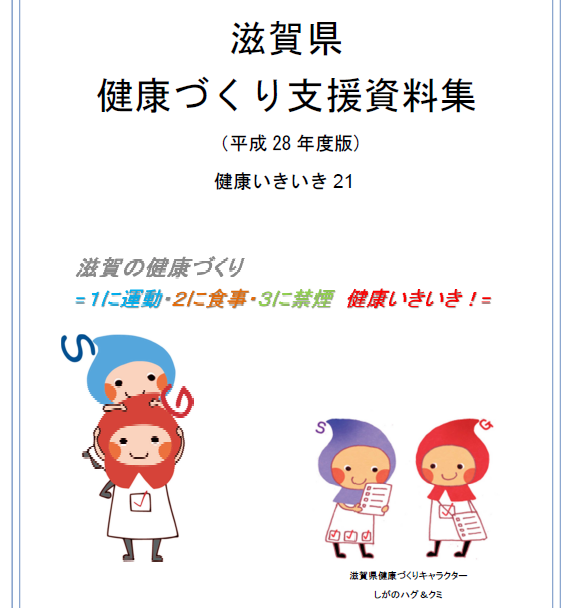
\includegraphics[ width=0.5\linewidth]{fig/fig12.png}
		%     \put(-0.7,0.5){滋賀県 女性, 12位}
		\caption{健康づくり支援資料集}\label{fig1}
	\end{center}
\end{figure}




%------------------------
\section{外部要因−社会・地理・環境の側面}
%------------------------

そのほか, 保健活動とは少し違う角度として, 滋賀県の各都市が便利で歩きやすい(コンパクトシティーである), スポーツなど健康的な娯楽がし易い, 災害が少ない, 気候が温暖, 平均収入が多くて持ち家率が高い(可処分所得が高い), 経済格差が少ない(ジニ係数が低い)などの環境要因も強く寄与しているのではないかと考えられる.


%------------------------
\section{リーダーの健康政策に関しての認識}
%------------------------
意思決定者の健康についての認識も事業の加速化に重要な部分である.
滋賀県では, 1993年度, 国松善次氏が健康福祉部長(1998年--2006年まで県知事)に就任した頃から,
健康づくり事業の重要性を認識し, 積極的に取り組むことになり, 様々な組織に対して支援を行った.
その間, 健康づくりには人や予算が十分に配分され, 滋賀県の現状に至る行政施策が推進されたとみられる.

%------------------------
\section{結論}
%------------------------
結局, 滋賀県では健康づくりのために特別な事業を行ったわけではなく,
\begin{itemize} \setlength{\itemsep}{-0.5mm} \setlength{\parskip}{-0.5mm}
	\item 組織 :  健康推進連絡協議会等活発な地域活動を支える組織があった.
	\item データの収集と情報公開 : 健康栄養マップ調査, 健康づくり支援資料集や死亡統計解析を作成することで, 県, 保健所, 市町が, 客観的データに基づいた健康づくり施策ができた.
	\item 市町への支援 : 保健所が市町の取り組みをうまく支援できた.
	\item 健康づくりに関心を持つ施策決定者の存在 : 健康づくりにきわめて熱心な施策決定者がいたことで, 組織に 人や予算がついた.
\end{itemize}
により, 健康づくりの基礎インフラが他県より進んでいたとも言える.

即ち, 健康づくりにおいて重要なのは, マクロ的視点で様々な角度から長期的な計画を立て,
\begin{itemize} \setlength{\itemsep}{-0.5mm} \setlength{\parskip}{-0.5mm}
	\item 「科学的根拠に基づいて」
	\item 「ヘルスプロモーションの理念に沿って地域活動を活性化」
	\item 「県, 保健所, 市町がそれぞれの役割に応じてPDCAサイクルを着実に実行」
\end{itemize}
のように, 正確な情報・持続性・協力体制を維持するのが重要だと考えられる.


%------------------------------------------------------------
\chapter{滋賀県の健康・平均寿命に関する公表結果}
%------------------------------------------------------------
\section{健康寿命の定義と算出方式}
\bb{健康寿命の概念を理解するためには, まず, 「疾病負荷(disease burden)」という概念を理解する必要がある. 疾病負荷とは疾病により失われた生命や生活の質の期間を意味する. 疾病負荷を計量化した指標の内, 近年最も広く使われている指標が障害調整生命年 (DALYs) である.
	ある人における障害調整生命年 (DALY, disability adjusted lit year) の計算は損失生存年数 (YLL, years of life lost) と障害生存年数 (YLD, years lived with disability)の合計
	$$DALY=YLL+YLD$$
	%「障害調整生命年 (DALY) = 損失生存年数 (YLL) + 障害生存年数 (YLD)」
	で計算され, 障害生存年数 (YLD)まで考慮した疾病負荷の指標である.
}

\begin{figure}[h!]
	\begin{center}
		%\includegraphics[ width=0.5\linewidth]{fig/daly.png}
		\caption{DALYの算出概念図, 出典:wikipedia.org, 障害調整生命年
		}
	\end{center}
\end{figure}


\bb{健康寿命はとは, 「健康上の問題で, 日常生活が制限されることなく生活できる期間」を意味し, 「生存年数(life year)- 障害生存年数 (YLD)」で定義される.
}

ある社会構成員における平均健康寿命と平均寿命\footnote{平均寿命は, 5年ごとの国勢調査で確定した人口とその年を含む前後3年間の死亡数をもとに, 厚生労働省により公表. 都道府県別, 市町村別,男女別に公表
}
との差を縮めることにより, 医療費や介護給付金の軽減, および個人の生活の質の低下を防ぐことができ, 社会が安定させることが出来る.
そのため, 健康寿命を延ばすこと, すなわち, 『健康寿命の延伸』が社会的に注目を集めている.
%
%健康寿命とは, 寿命期間の内, 健康上の問題で日常生活が制限されることなく 自立して生活できる期間をいう.

現在, 健康寿命の算出方式は主に,
\begin{itemize} \setlength{\itemsep}{-0.5mm} \setlength{\parskip}{-0.5mm}
	\item 国民生活基礎調査でのアンケート項目\footnote{
		      統計調査の調査票(健康表)
		      \url{http : //www.mhlw.go.jp/toukei/chousahyo/index.html#00450061}.
	      }
	      より算出
	      \begin{itemize} \setlength{\itemsep}{-0.5mm} \setlength{\parskip}{-0.5mm}
		      \item 例) あなたは, 現在, 傷病で病院や診療所に通ってますか.
		            \begin{itemize} \setlength{\itemsep}{-0.5mm} \setlength{\parskip}{-0.5mm}
			            \item[] 1. 通っている~~~~~~2. 通っていない
		            \end{itemize}
	      \end{itemize}

	\item 介護保険の要介護認定率より算出
	      \begin{itemize} \setlength{\itemsep}{-0.5mm} \setlength{\parskip}{-0.5mm}
		      \item 要介護2以上を不健康とするもの
	      \end{itemize}
\end{itemize}
2種類のデータから算出される.\footnote{
	健康寿命算出プログラム
	\url{http : //toukei.umin.jp/kenkoujyumyou/}.
}
二つの方法の内, 介護保険に基づいた後者の方式は,
ほぼすべての県民が介護保険の対象となっていること, 全国同一
の基準で判定されていることから, 客観的で信頼度の高い数値ととらえる.

\section{滋賀県の平均寿命}
平均寿命とは0歳の平均余命を意味する。
厚生労働省\footnote{
	厚労省都道府県別生命表
	\url{http://www.mhlw.go.jp/toukei/saikin/hw/seimei/list54-57-02.html}}により2010年度の平均寿命では,
男性の場合, 長野県が 80.88歳で1位を示し, その次が滋賀県(80.58歳)であった. 47都道府県の内, 平均寿命80歳以上の県は,
上位から長野, 滋賀,  福井, 熊本,  神奈川,   京都,   奈良,   大分の順位であった.

\begin{figure}[h!]
	\begin{center}
		%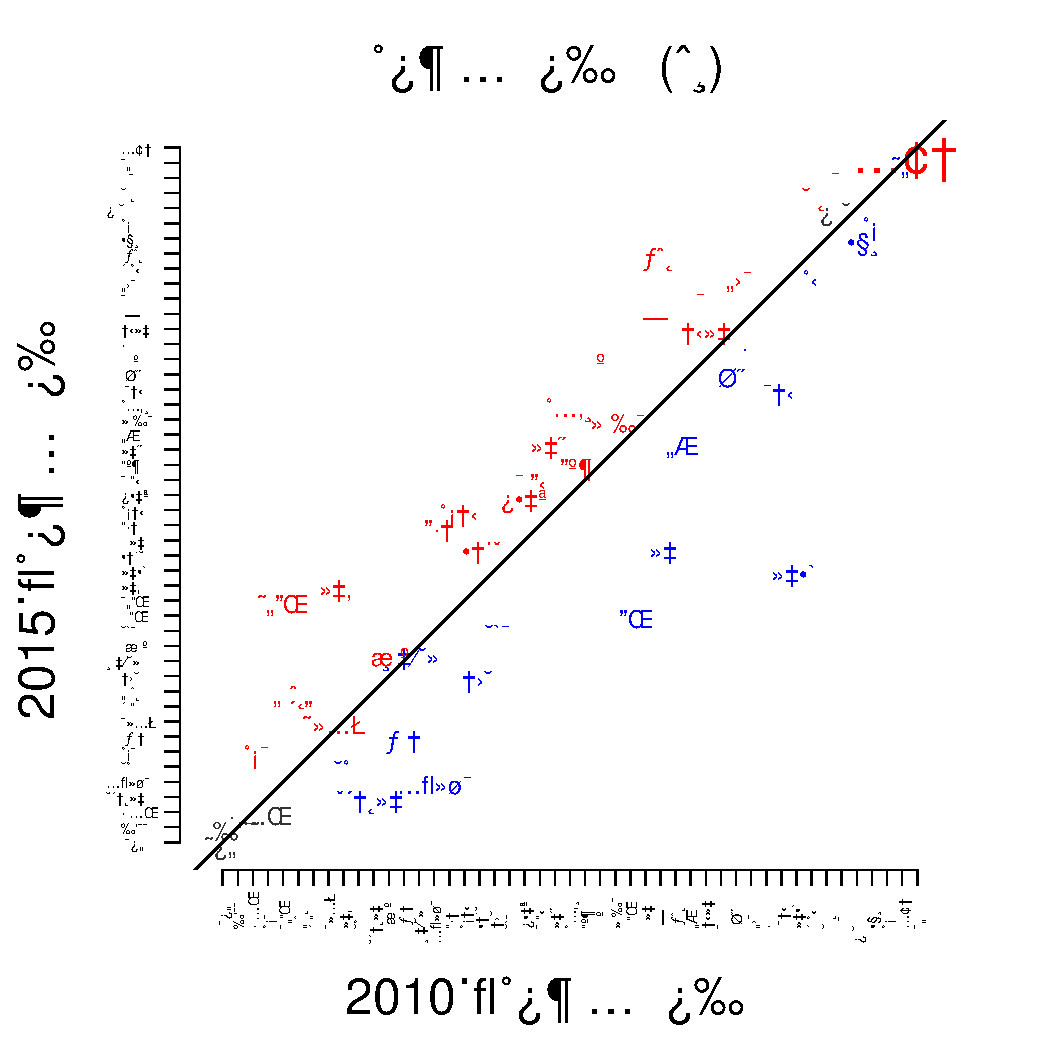
\includegraphics[ width=0.49\linewidth]{fig/rankmale.pdf}
		%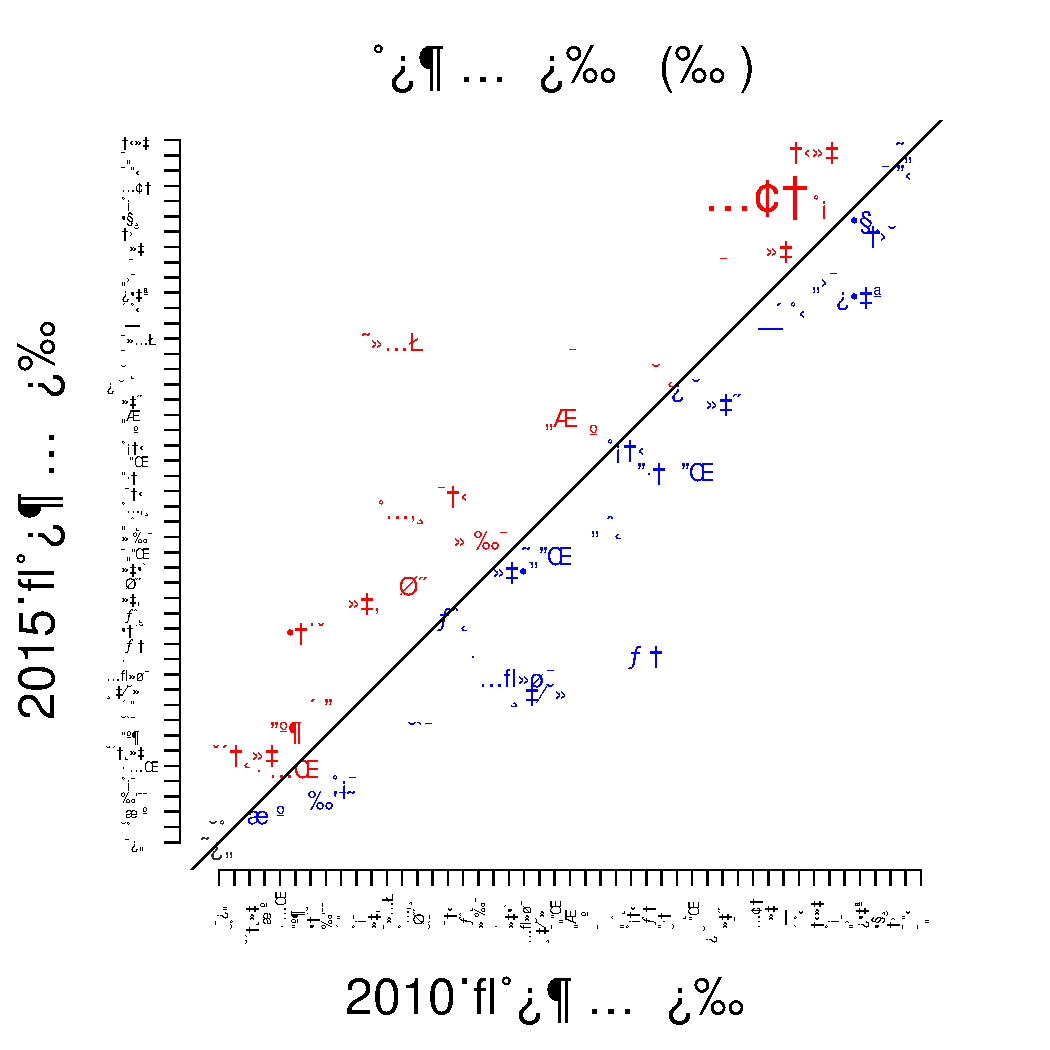
\includegraphics[ width=0.49\linewidth]{fig/rankfemale.pdf}
		%     \put(-0.1,0.9){滋賀県 男性, 2位}
		\caption{都道府県別平均寿命順位推移(2010年〜2015年, 男)}
	\end{center}
\end{figure}

% \begin{figure}[h!]
%\begin{center}
%    %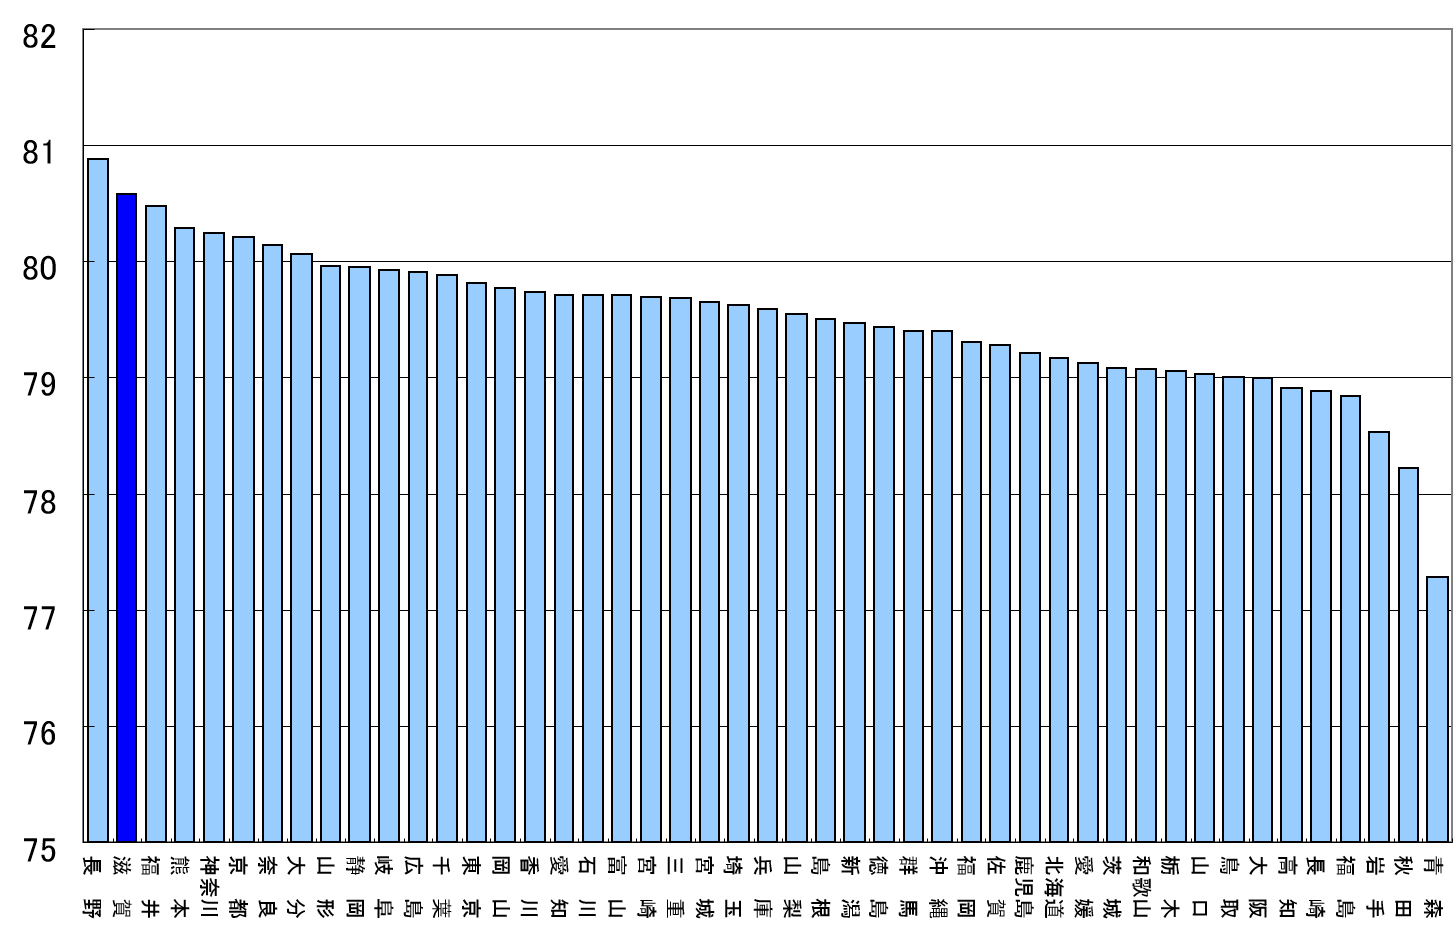
\includegraphics[ width=0.5\linewidth]{fig/fig1.png}
%     \put(-0.9,0.5){滋賀県 男性, 2位}
%\caption{都道府県別平均寿命(2010年, 男)}\label{fig1 }
%\end{center}
%\end{figure}

同年度の女性の場合, 全ての県が85歳を超えている結果となった.
男性と同じく長野県が1位を示し, 滋賀県の女性の平均寿命は12位を示している.
上位から長野, 島根, 沖縄, 熊本, 新潟, 広島, 福井, 岡山, 大分, 富山, 石川, 滋賀の順位であった.
男女ともに, 青森県の平均寿命は全国で最下位を示している.
\begin{figure}[h!]
	\begin{center}
		%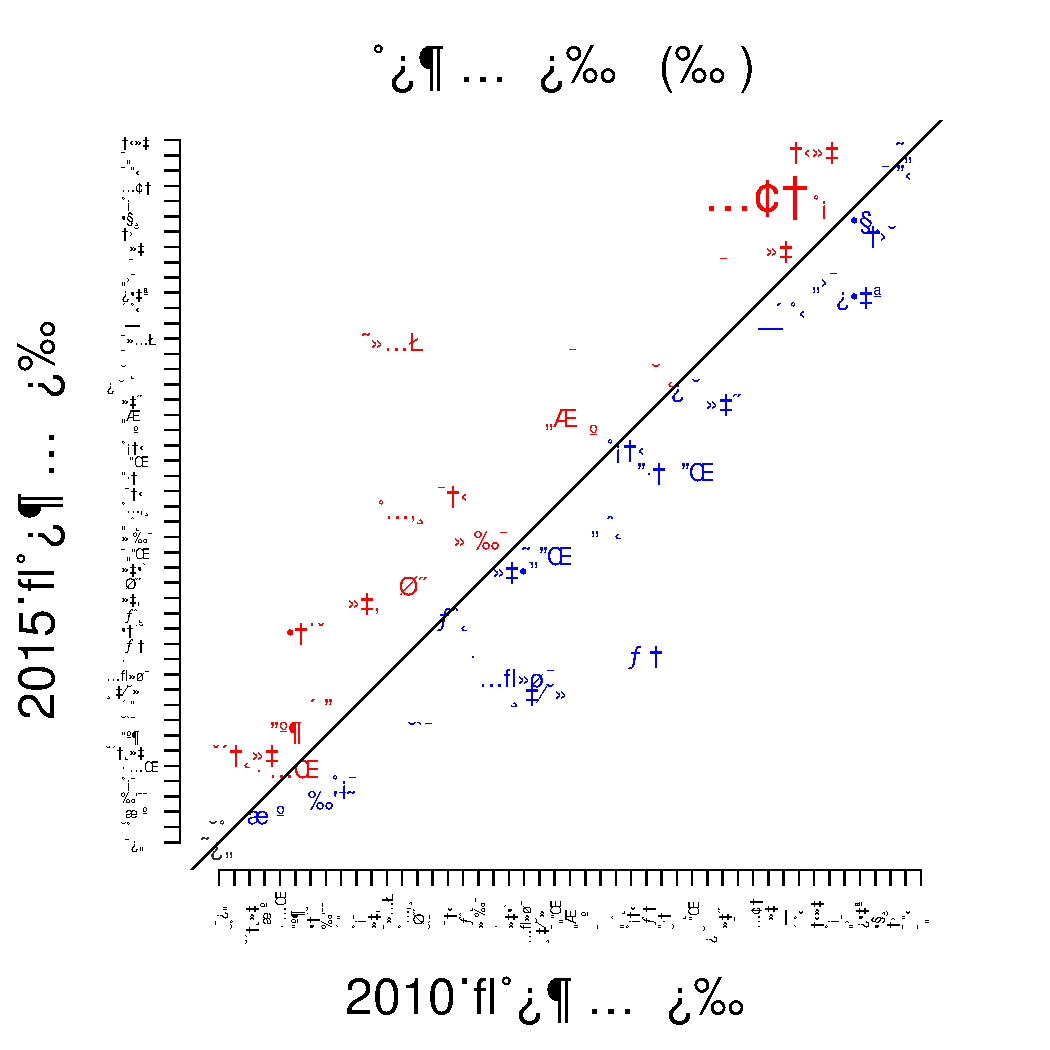
\includegraphics[ width=0.5\linewidth]{fig/rankfemale.pdf}
		%     \put(-0.1,0.9){滋賀県 男性, 2位}
		\caption{都道府県別平均寿命順位推移(2010年〜2015年, 女)}\end{center}
\end{figure}


%\begin{figure}[h!]
%\begin{center}
%    %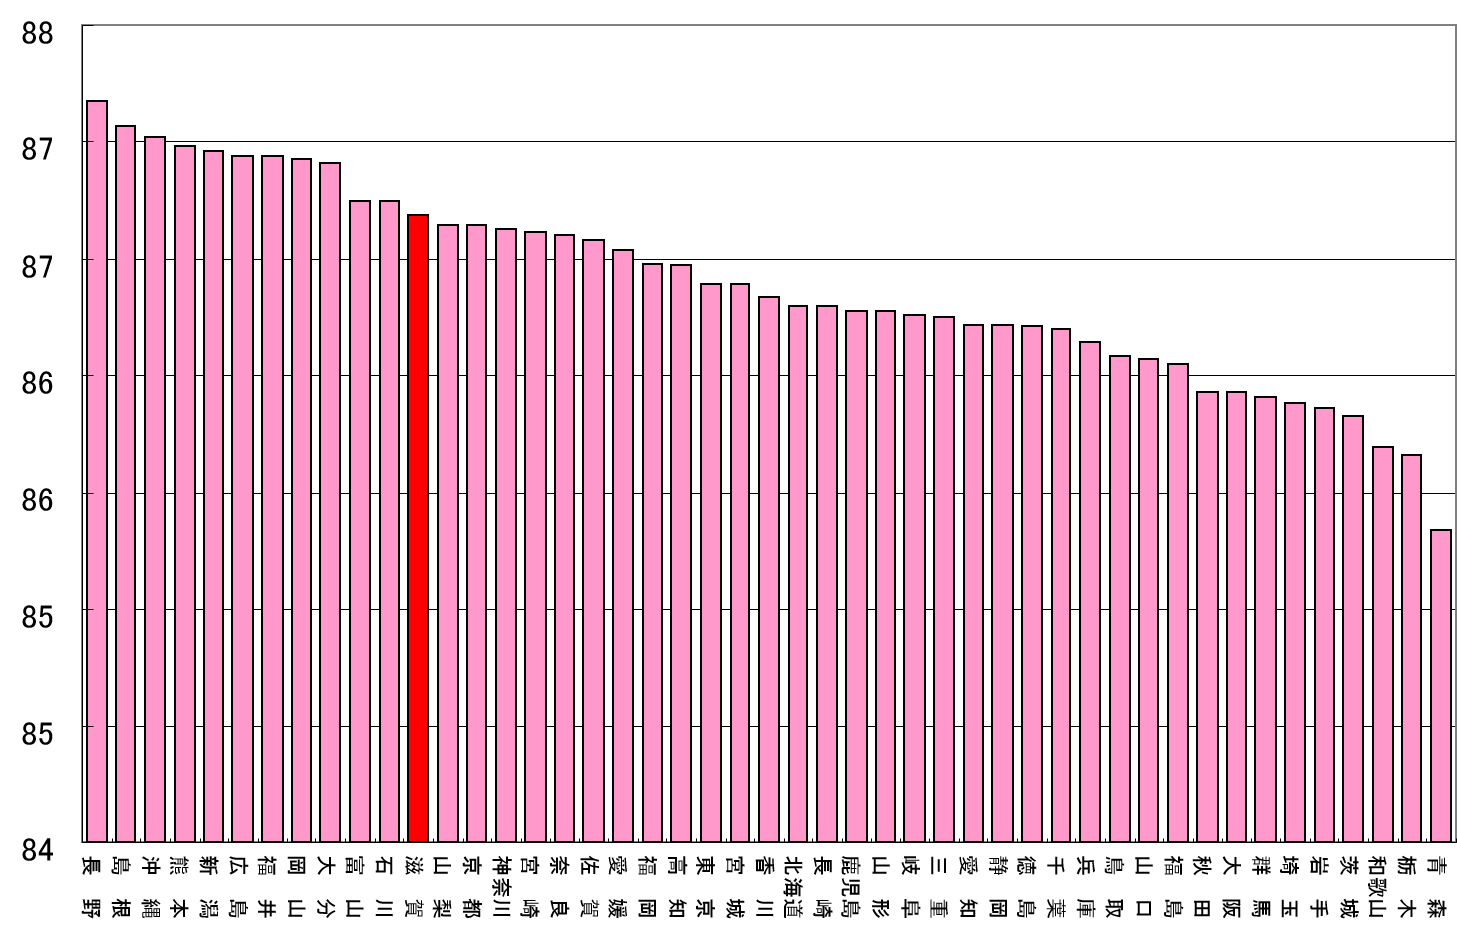
\includegraphics[ width=0.5\linewidth]{fig/fig2.png}
%     \put(-0.7,0.5){滋賀県 女性, 12位}
%   \caption{都道府県別平均寿命(2010年, 女)}\label{fig1}
%\end{center}
%\end{figure}
%
\begin{figure}[h!]
	\begin{center}
		%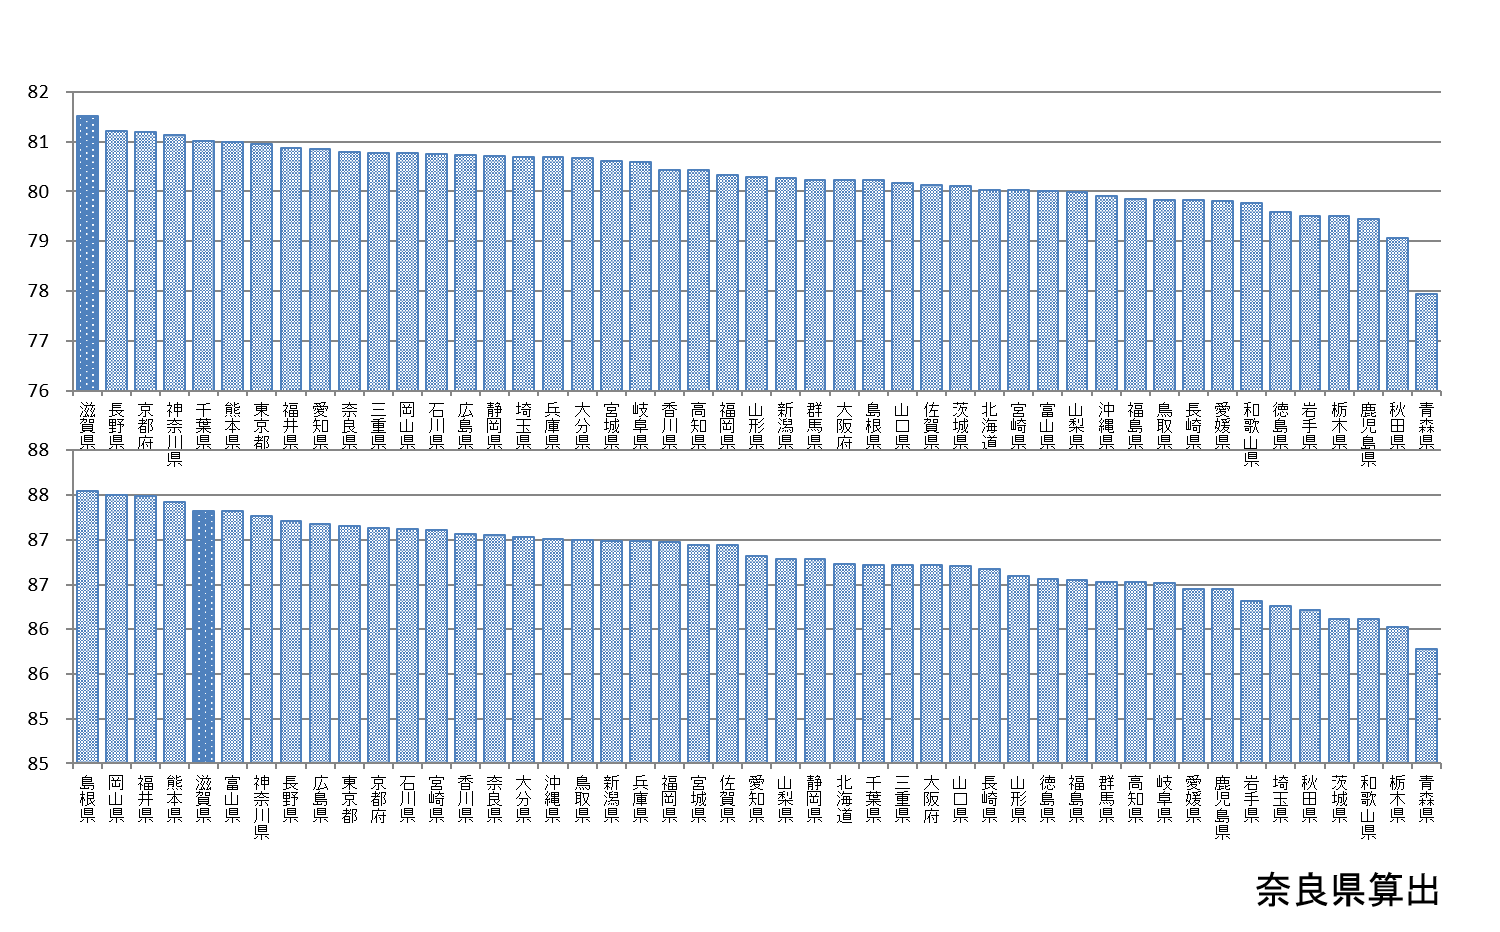
\includegraphics[ width=0.5\linewidth]{fig/fig6.png}
%		\put(-0.9,0.55){滋賀県 男性, 1位}
%		\put(-0.85,0.25){滋賀県 女性, 5位}
		\caption{滋賀県民の平均寿命(2014年, 奈良県算出)}\label{fig1}
	\end{center}
\end{figure}



\begin{figure}[h!]
	\begin{center}
		%    %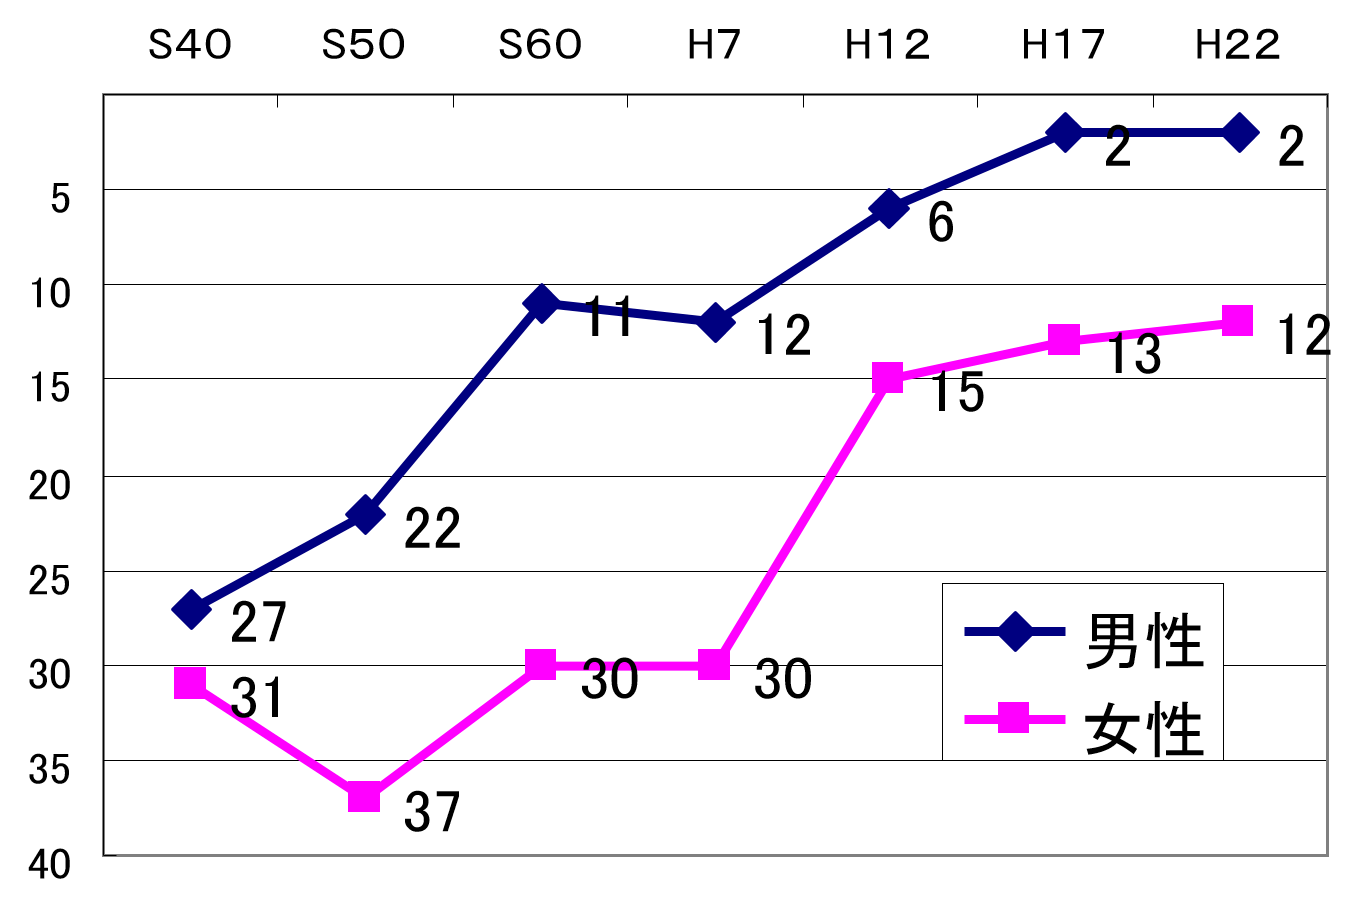
\includegraphics[ width=0.5\linewidth]{fig/fig3.png}
		%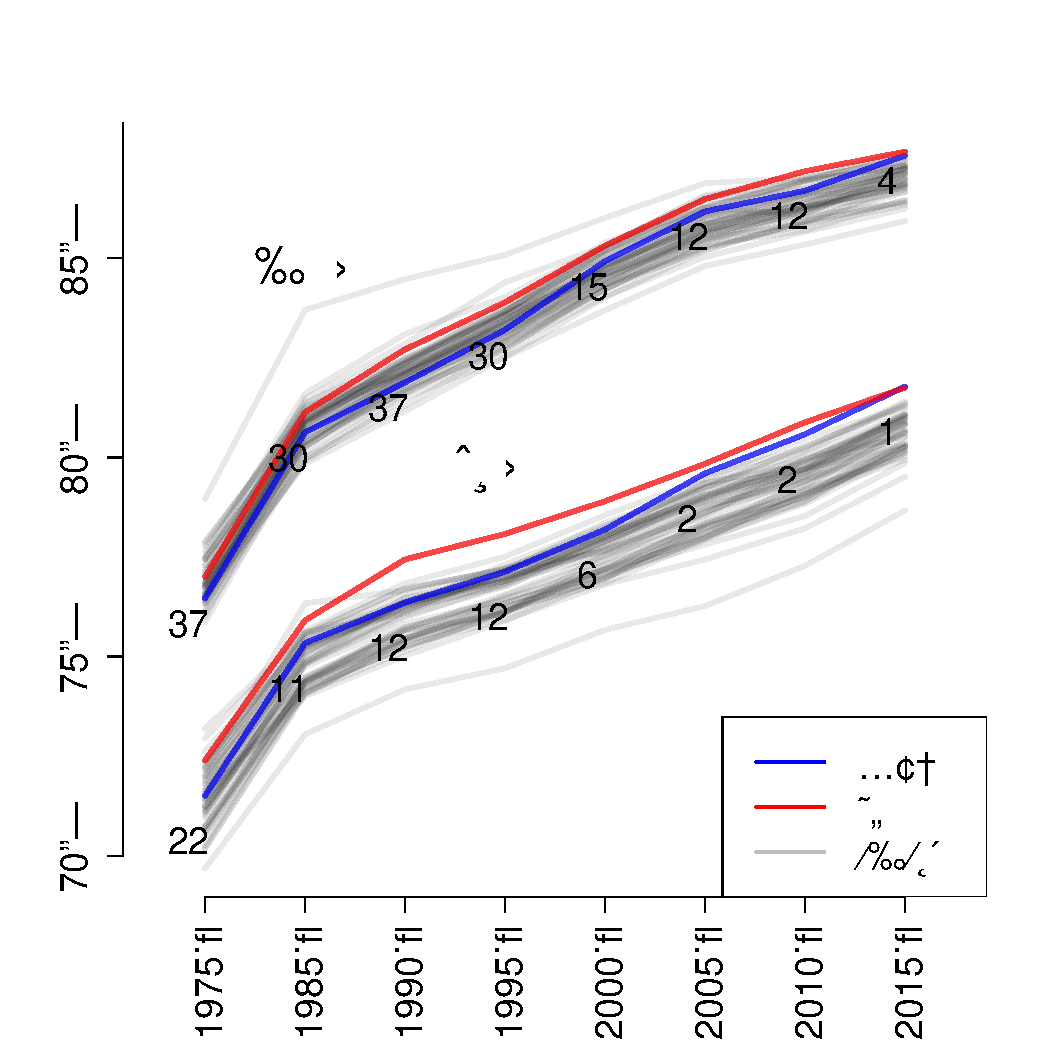
\includegraphics[ width=0.5\linewidth]{fig/fig3pdf.pdf}
		%     \put(-0.7,0.5){滋賀県 女性}
		\caption{平均寿命の延伸と滋賀県の都道府県順位推移}
	\end{center}
\end{figure}
%\begin{figure}[h!]
%\begin{center}
%    %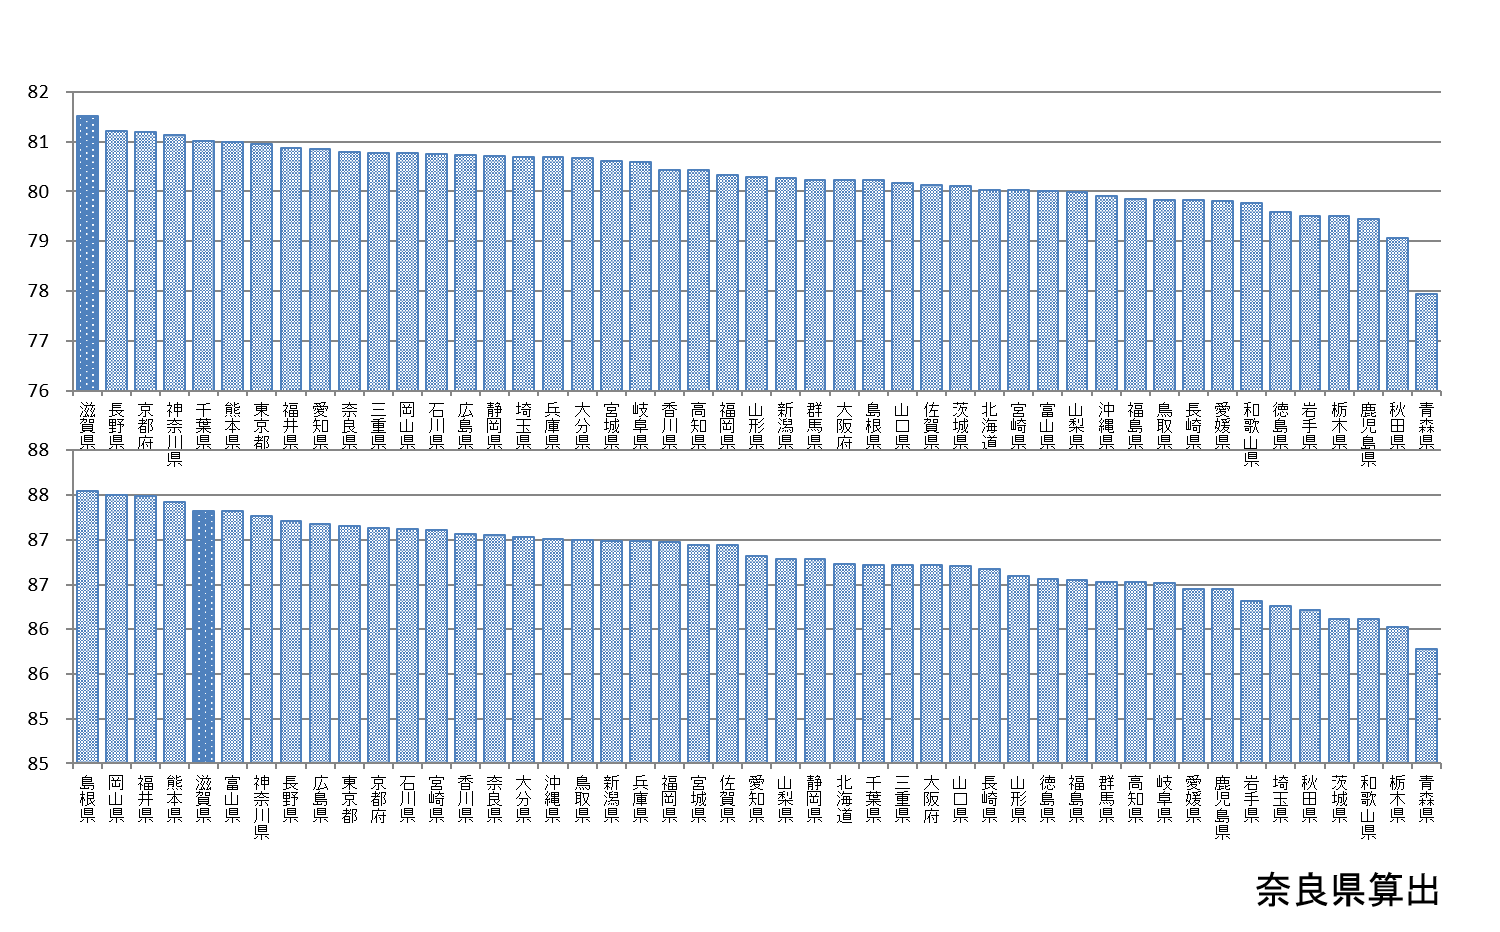
\includegraphics[ width=0.5\linewidth]{fig/fig6.png}
%%     \put(-0.7,0.5){滋賀県 女性}
%   \caption{滋賀県民の平均寿命 奈良県算出}\label{fig1}
%\end{center}
%\end{figure}
%
2014年度, 奈良県が算出した平均寿命によると, 男性は全国1位, 女性は全国5位となった.

滋賀県の平均寿命は都道府県順位の推移をみると,
60年代から持続的に上がってきたことがわがる.

これは, 滋賀県が長寿県になったのは単なる横断(cross-sectional)データから見られる一時的現象ではなく, 縦断(longitudinal)データからも立証されたことを意味する.

滋賀県の平均寿命を19市町別にみると, 男性は愛荘町, 女性は豊郷町が本県内で長寿地域であった.
\begin{figure}[h!]
	\begin{center}
		%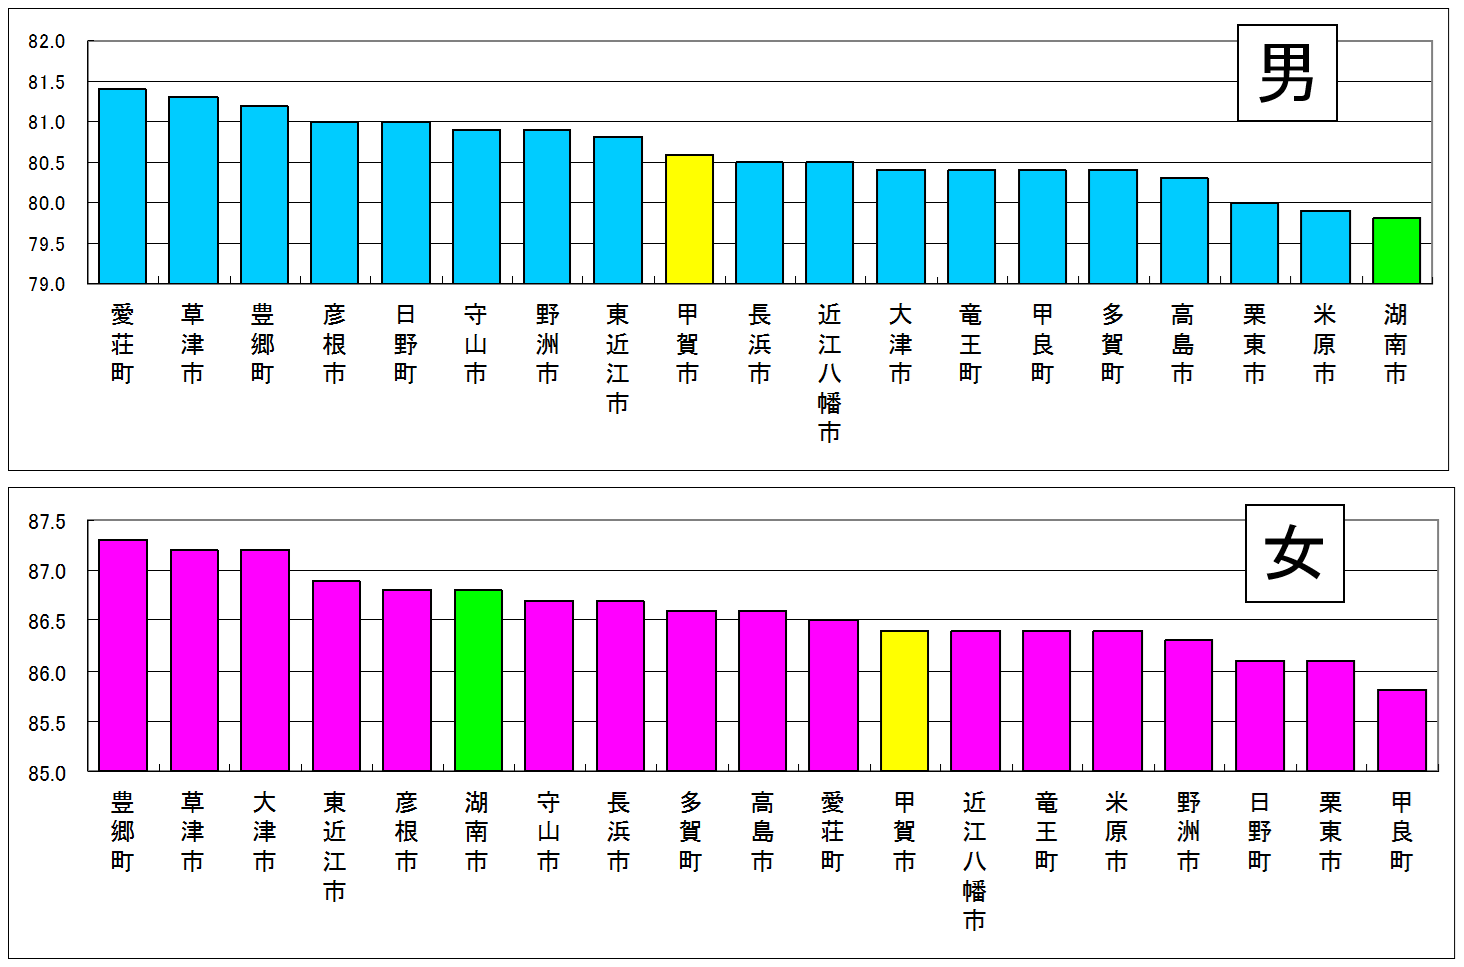
\includegraphics[ width=0.5\linewidth]{fig/fig4.png}
		%     \put(-0.7,0.5){滋賀県 女性}
		\caption{市町別平均寿命(2010年, 男女)}\label{fig1}
	\end{center}
\end{figure}


%------------------------------------------------------------
\section{滋賀県の健康寿命(要介護度方式)}
%------------------------------------------------------------
\subsection{介護保険制度と要支援・要介護度}
健康寿命の要介護度方式による算出方式は, 要介護度を利用するため, 介護保険制度と要介護度の概念を整理しておく.

介護保険制度は社会保険制度\footnote{一般的に医療, 年金, 介護保険を指す. 広義の定義では雇用, 労災保険まで含む.
	%https : //hoken.azukichi.net/shaho.html#1
}の一つとして,
高齢者や, 介護が必要な人に対する保障制度である.
40歳以上の人に加入が義務付けられている.\footnote{
	現在の介護保険制度は, 1997年に制定され, 2000年4月1日に施行された介護保険法(平成9年法律第123号)に基づいて実施されている.
}
%高齢者の介護を保障する制度である.


保険給付を受けるにあたって, 被保険者は市町村に申請して認定を受けなければならない.
認定を受けられる被保険者は, 65歳以上の人もしくは, 4064歳までで加齢が原因と思われる「特定疾病(16種類)」の人となる.
判定は下記の手順でおこなう.
\begin{itemize} \setlength{\itemsep}{-0.5mm} \setlength{\parskip}{-0.5mm}
	\item 1次判定  :  訪問調査, コンピュータにより判定
	      \begin{itemize} \setlength{\itemsep}{-0.5mm} \setlength{\parskip}{-0.5mm}
		      \item 申請者の心身の状況, 置かれている環境等について, 全国一律の基準に基づいて訪問調査
	      \end{itemize}
	\item 被保険者の主治医に対して, 被保険者の疾病や負傷の状況等について意見を聞き取り
	\item 2次判定  :  介護認定審査会により判定
	      %市町村の(保健・医療・福祉の専門家により構成)は,
	      \begin{itemize} \setlength{\itemsep}{-0.5mm} \setlength{\parskip}{-0.5mm}
		      \item 訪問調査結果(1次判定)や主治医の意見等をもとに審査・判定を行い, その結果を市町村に通知
	      \end{itemize}
\end{itemize}
市町村は, 介護認定審査会(保健・医療・福祉の専門家により構成)の2次判定結果に基づいて要支援・要介護認定を行う.

\subsection{要支援・要介護認定の結果}
要支援・要介護認定は7段階で構成されており,  要支援は2段階, 要介護は5段階ある.
%要支援・要介護は段階によって分かれており,
それぞれの段階において利用できる介護サービスの範囲や量, 負担料金の上限が決まる.

\begin{itemize} \setlength{\itemsep}{-0.5mm} \setlength{\parskip}{-0.5mm}
	\item 要支援1  :  支給限度額 :5万30円/月
	      \begin{itemize} \setlength{\itemsep}{-0.5mm} \setlength{\parskip}{-0.5mm}
		      \item 日常生活上の基本動作については, ほぼ自分で行うことが可能だが, 要介護状態への進行を予防するために, IADL(手段的日常生活動作)において何らかの支援が必要な状態.
	      \end{itemize}

	\item 要支援2  :  支給限度額 :10万4730円/月

	      \begin{itemize} \setlength{\itemsep}{-0.5mm} \setlength{\parskip}{-0.5mm}
		      \item 要支援1と比べて, IADL(手段的日常生活動作)を行う能力がわずかに低下し, 機能の維持や改善のために何らかの支援が必要な状態.

	      \end{itemize}

	\item 要介護1 : 支給限度額 :16万6920円/月


	      \begin{itemize} \setlength{\itemsep}{-0.5mm} \setlength{\parskip}{-0.5mm}
		      \item 要支援の状態からさらにIADL(手段的日常生活動作)の能力が低下. 排せつや入浴などに部分的な介護が必要な状態.

	      \end{itemize}

	\item 要介護2 : 支給限度額 :19万6160円/月


	      \begin{itemize} \setlength{\itemsep}{-0.5mm} \setlength{\parskip}{-0.5mm}
		      \item 要介護1の状態に加えて, 歩行や起き上がりなどに部分的な介護が必要な状態.

	      \end{itemize}

	\item 要介護3 : 支給限度額 :26万9310円/月


	      \begin{itemize} \setlength{\itemsep}{-0.5mm} \setlength{\parskip}{-0.5mm}
		      \item 要介護2の状態からさらにIADL(手段的日常生活動作)およびADL(日常生活動作)が著しく低下し, 立ち上がりや歩行が自力ではできず, 排泄や入浴, 衣服の着脱などにもほぼ全面的な介護が必要な状態.

	      \end{itemize}

	\item 要介護4 : 支給限度額 :30万8060円/月


	      \begin{itemize} \setlength{\itemsep}{-0.5mm} \setlength{\parskip}{-0.5mm}
		      \item 要介護3よりも動作能力が著しく低下し, 日常生活ほぼ全般を介護なしで行うことが困難な状態.

	      \end{itemize}

	\item 要介護5 : 支給限度額 :36万650円/月


	      \begin{itemize} \setlength{\itemsep}{-0.5mm} \setlength{\parskip}{-0.5mm}
		      \item 要介護4の状態よりさらに動作能力が低下し, 意思の伝達も困難になり, 介護なしには日常生活を送ることが不可能な状態.

	      \end{itemize}


\end{itemize}


%いずれかの区分に認定されたのちに, 介護保険サービスを利用することができます.



%要支援・要介護とは, 介護サービスを受ける際に, その状態がどの程度なのかを判定するものです.






%申請を受けた市町村は, 申請者の心身の状況, 置かれている環境等について, 全国一律の基準に基づいて訪問調査を行い, コンピュータにより判定する(1次判定). また, 市町村は, 被保険者の主治医に対して, 被保険者の疾病や負傷の状況等について意見を求める. 市町村の介護認定審査会(保健・医療・福祉の専門家により構成)は, 訪問調査結果や主治医の意見等をもとに審査・判定を行い, その結果を市町村に通知する(2次判定).

%認定は, 原則として申請日から30日以内に行われる.
%認定の効力は申請日にさかのぼり, 申請日以降に利用したサービスについて給付が受けられる. 認定には有効期間が設定され, 定期的に更新される. また, 有効期間内であっても要支援・要介護状態に変化があった場合は, 被保険者の申請または市町村の職権により, 変更の認定, 認定の取消し等を行うことができる.
%となっています.
%




%\footnote{国際的には, ドイツ, 韓国などは日本と同様に社会保険方式を採用しているが, イギリス, スウェーデンなどは一般税財源による社会サービス方式を採用している.
%}
%高齢者や, 老化で介護が必要な人に対する保障制度で, 40歳以上の人に加入が義務付けられています.
%訪問介護や老人福祉施設の利用などの各種サービスを受けられます.

%保険料は, 65歳未満の人は健康保険や国民健康保険などの医療保険に含まれる形になっています. 65歳以上になると医療保険と切り離され, 原則として年金から天引きされます.

%以下は,
%
%日本の介護保険制度の概要である
%要介護度の基準は厚生労働省が決めている.

%以下参考にしてください


%
%
%
\subsection{滋賀県の健康寿命結果}
介護度による健康寿命は前述した「要介護の2以上」を不健康状態に定義し, それに基づいて計算される. 介護度に基づいた健康寿命は「平均自立期間」とも呼ばれる.\footnote{厚生労働科学研究健康寿命のページ(\url{http://toukei.umin.jp/kenkoujyumyou/}).
	「健康寿命の指標化に関する研究」
}
\begin{figure}[h!]
	\begin{center}
		%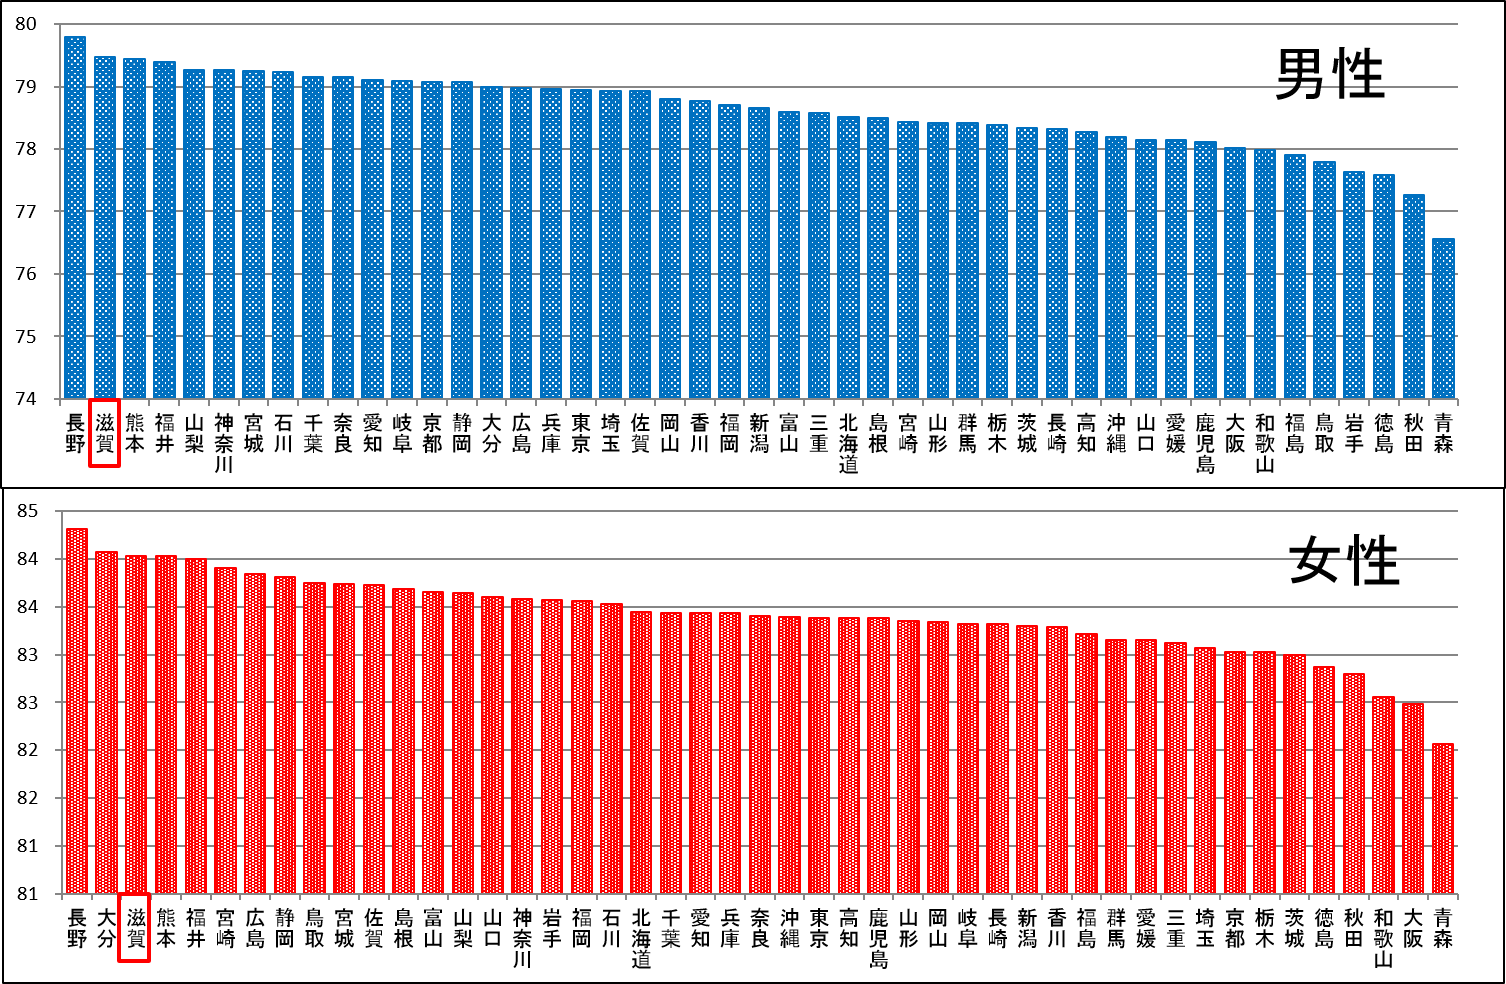
\includegraphics[ width=0.5\linewidth]{fig/fig5.png}
%		\put(-0.92,0.6){$\leftarrow$滋賀県 男性 2位}
%		\put(-0.90,0.25){$\leftarrow$滋賀県 女性 3位}
		\caption{都道府県別健康寿命(平均自立期間, 2013年)}\label{fig1}
	\end{center}
\end{figure}
\begin{figure}[h!]
	\begin{center}
		%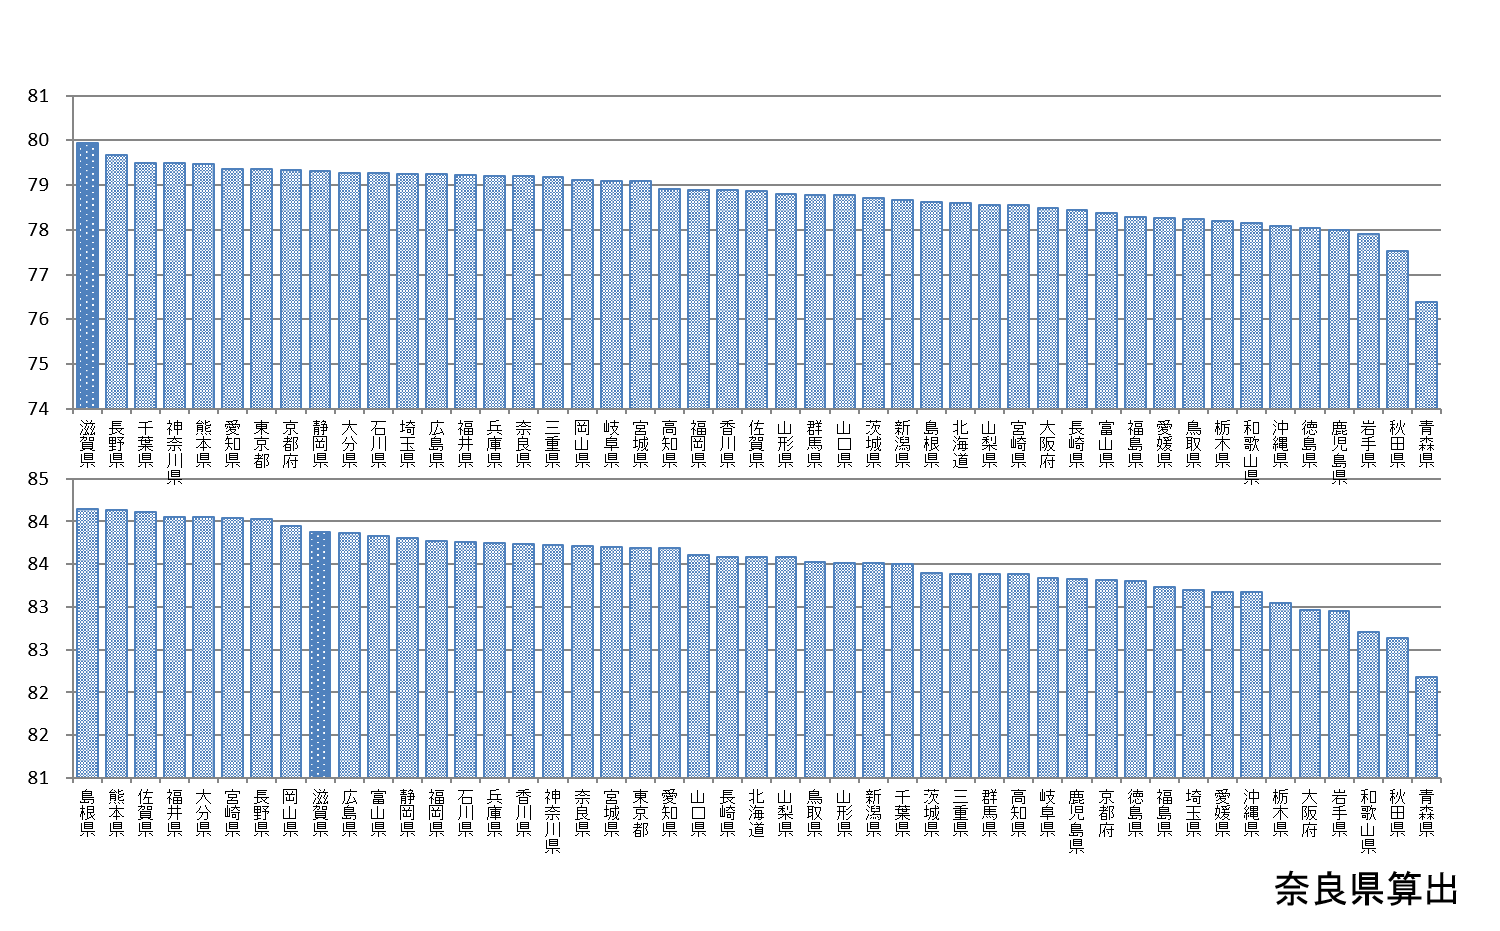
\includegraphics[ width=0.5\linewidth]{fig/fig7.png}
%		\put(-0.9,0.5){$\leftarrow$滋賀県 男性 1位}
%		\put(-0.75,0.25){$\leftarrow$滋賀県 女性 9位}
		\caption{都道府県別健康寿命(平均自立期間, 2014年)}\label{fig1}
	\end{center}
\end{figure}
次の図にこの方式に基づいた2013年と2014年の全国都道府県の健康寿命の結果を示す.

いずれも滋賀県の男性は両年度それぞれ2位と1位, 女性は3位と9位を示しており, 滋賀県が量的な指標(平均寿命)のみならず, 質の高い健康な県であることを示している.

後述するアンケート方式の健康寿命の算出方法は,
都道府県別の分析のみ可能だが,
要介護度方式は市町ごとまで分析できるのがもう一つの利点である.
次の図に県内19市町の健康寿命の分布を示す. 男性の場合は草津市, 女性の場合は日野町の健康寿命がもっとも長かった.

\begin{figure}[h!]
	\begin{center}
		%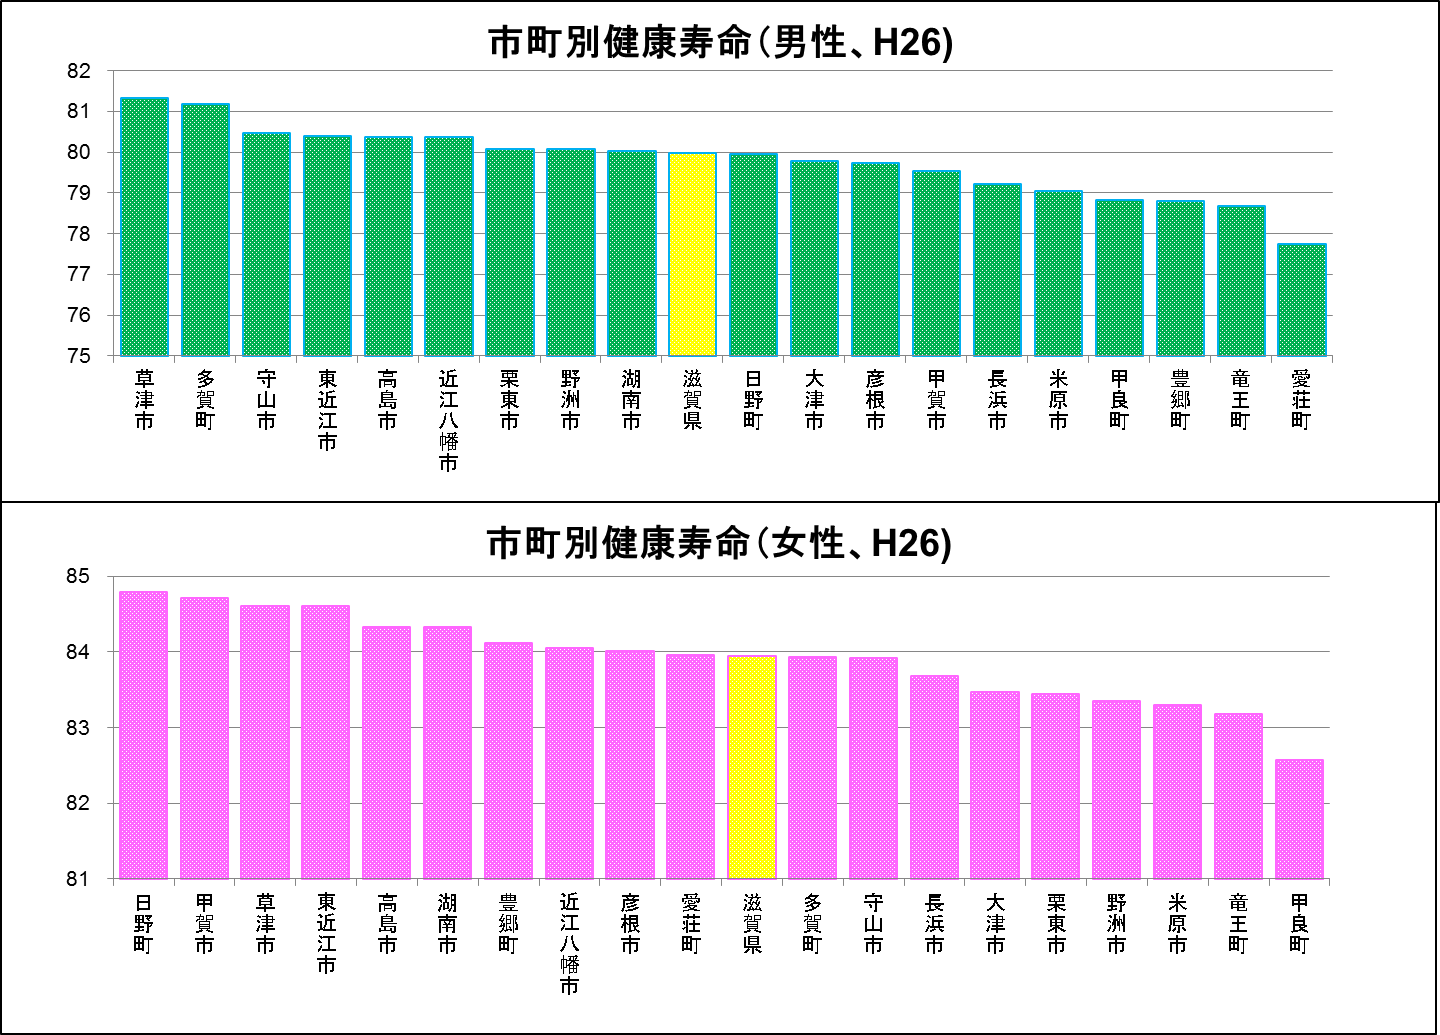
\includegraphics[ width=0.5\linewidth]{fig/fig8.png}
		% \put(-0.9,0.65){$\leftarrow$草津市}
		% \put(-0.9,0.3){$\leftarrow$日野町}
		\caption{滋賀県市町別健康寿命(2014年)}\label{fig1}
	\end{center}
\end{figure}



%------------------------------------------------------------
\section{滋賀県の健康寿命(アンケート方式)}
%------------------------------------------------------------
アンケートによる健康寿命は,
国民生活基礎調査でのアンケート項目により算出する.
国民生活基礎調査のアンケート項目とは,

\begin{itemize} \setlength{\itemsep}{-0.5mm} \setlength{\parskip}{-0.5mm}
	\item  例) あなたは, 現在, 傷病で病院や診療所に通ってますか.
	      \begin{itemize} \setlength{\itemsep}{-0.5mm} \setlength{\parskip}{-0.5mm}
		      \item 1. 通っている~~~~~~2. 通っていない
	      \end{itemize}
\end{itemize}
との質問に「通っている」と答えた人を不健康である
と定義する.
この方法は自己申告という主観的な回答である
ことから, 県民性に強く影響を受けるとともに
, 例えば, 滋賀県の場合, 県民約1,300人を対象とした調査の結果なので, この程度の人数では算出された値の信頼度が低いという欠点がある.
%\begin{tikzpicture}
%    %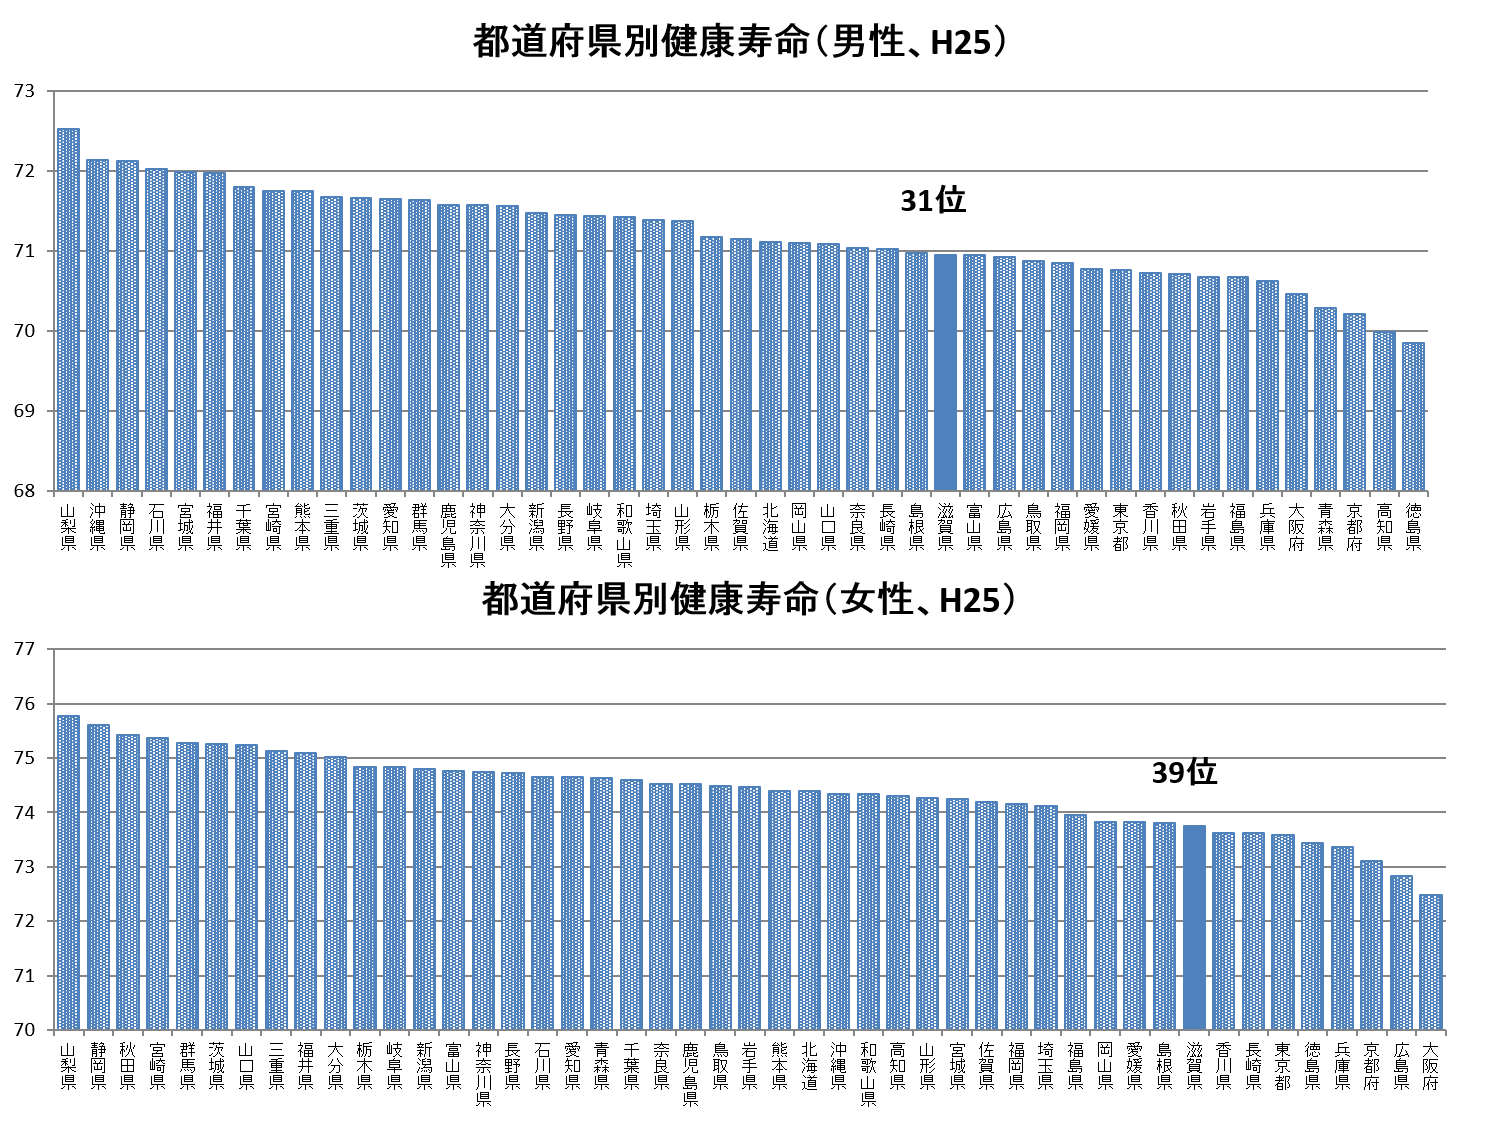
\includegraphics[ width=0.5\linewidth]{fig/fig9.png}
%\draw[step=0.1\linewidth,gray,very thin](-1,0) grid (0,0);
%\end{tikzpicture}

\begin{figure}[h!]
	\begin{center}
		%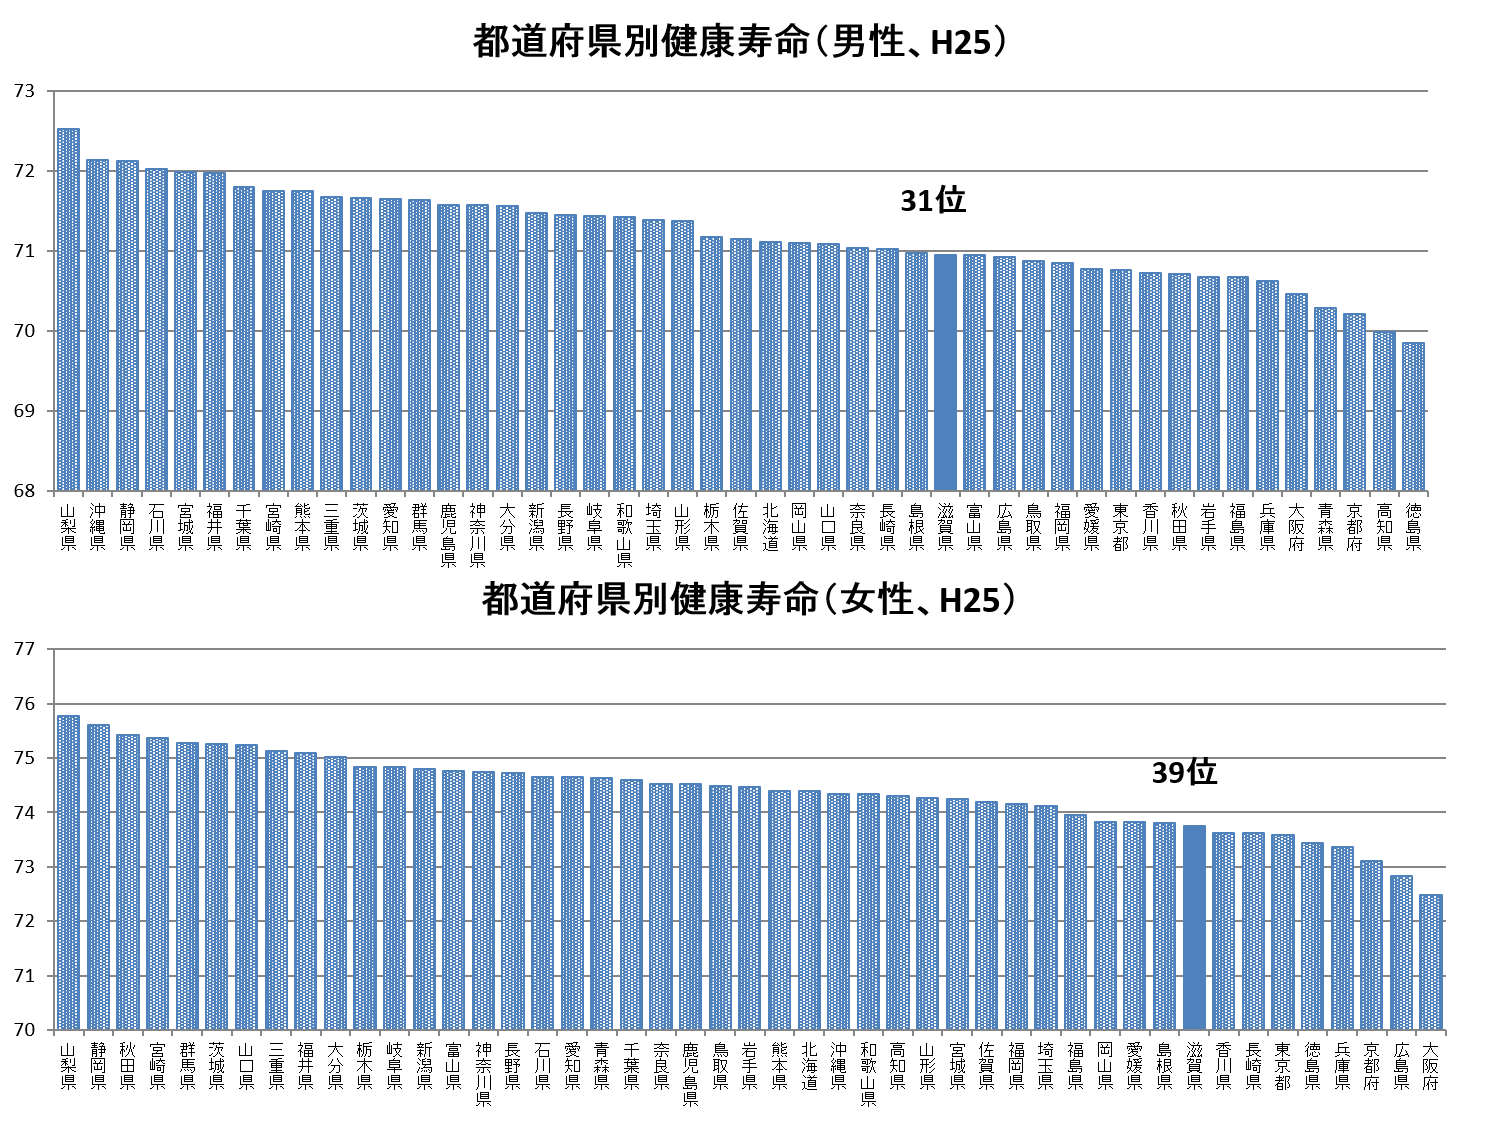
\includegraphics[ width=0.5\linewidth]{fig/fig9.png}
		% \put(-0.3,0.6){$\leftarrow$男 31位}
		% \put(-0.2,0.25){$\leftarrow$女 39位}
		\caption{都道府県別アンケート方式健康寿命(2013年)}\label{fig1}
	\end{center}
\end{figure}

アンケート方式の滋賀県の健康寿命は男性31位, 女性39位を示しており, 要介護方式の結果とはやや相反している結果となった.
こうした両方式の違いがなぜ生じたのかはまだ不明であるが, 上述したように, アンケートに当たって, サンプリング方法の問題,
サンプルの数などの疑問に加え, 県民性による偏りなどが考えられる.
%------------------------------------------------------------
\section{滋賀県の健康-国際研究資料にもとづいて}
%https://www.nikkei.com/article/DGXLRSP451461_Y7A710C1000000/
%http://release.nikkei.co.jp/attach_file/0451461_01.pdf
%https://www.nikkei.com/article/DGXLASDG19H77_Q7A720C1CR0000/
\begin{figure}[h!]
	\begin{center}
		%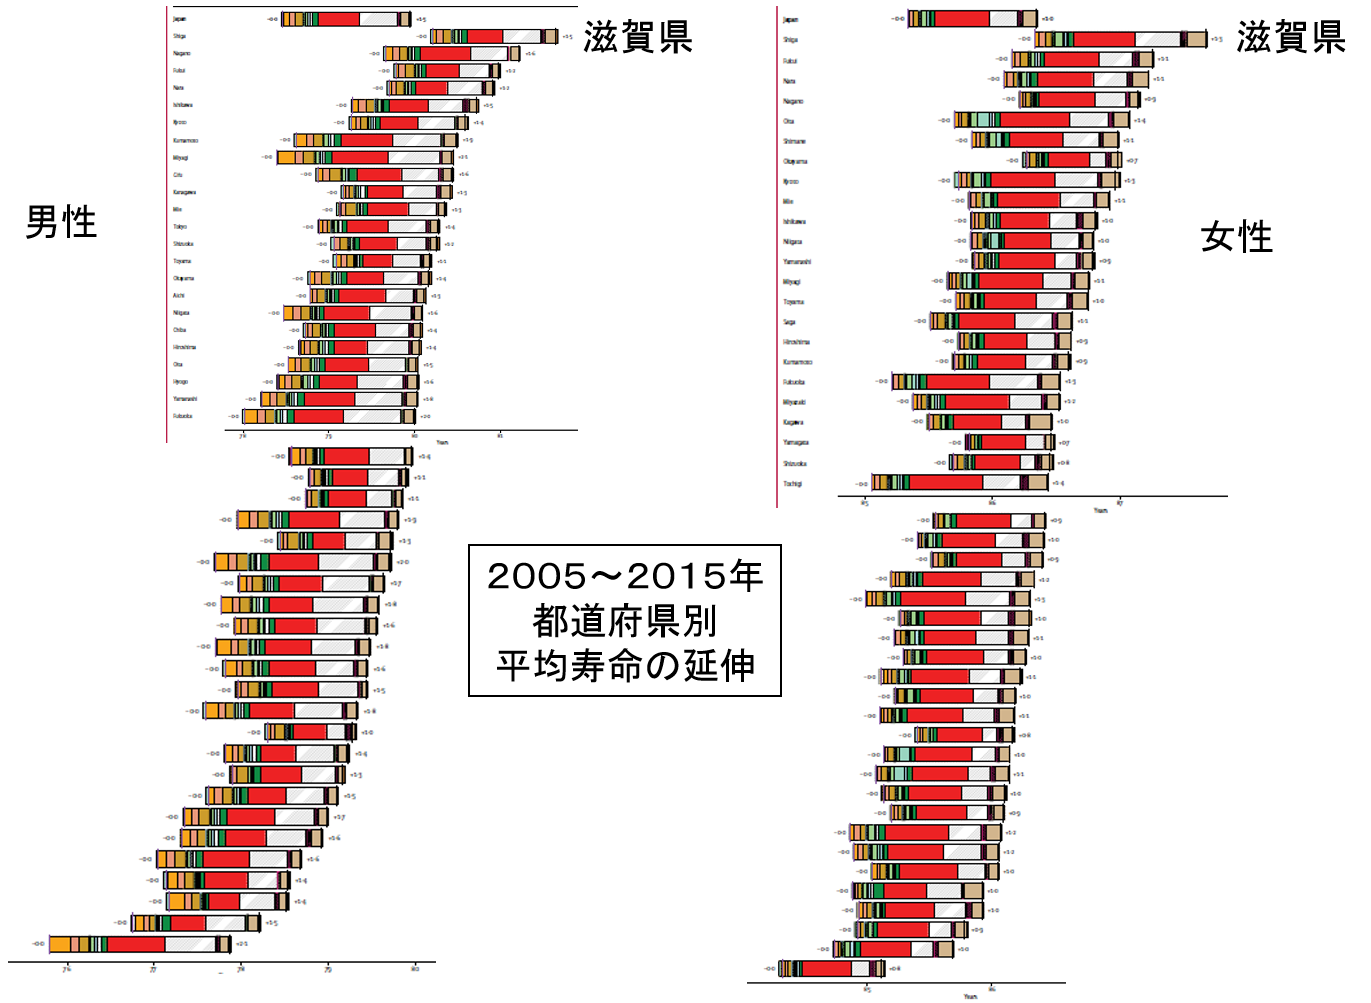
\includegraphics[ width=0.5\linewidth]{fig/fig10.png}
		%     \put(-0.3,0.65){$\leftarrow$草津市}
		%     \put(-0.3,0.3){$\leftarrow$日野町}
		\caption{平均寿命の延伸(2005〜2015年)}\label{fig10}
	\end{center}
\end{figure}

英医学誌ランセットに掲載された野村ら(2017)の研究でも, 滋賀県が健康県であることが示された.
この研究では, 1990 年〜 2015 年における日本の健康指標の変化, 及び 都道府県別の健康指標の改善状況について包括的な分析を行った. その結果, 男女合わせた日本人の平均寿命が
同時期に延伸された傾向が確認されている他, 特に, 滋賀県の平均寿命が2015年度において都道府県の中でも最も長い, 長寿県となっていることが明らかになった(図\ref{fig10}).
%
%
%1990年の79.0歳から2015年の83.2歳まで4.2歳上昇した結果であった



%健康寿命も1990年に最も長い長野県(71.5歳)と最も短い高知県(69.2歳)の差は2.3歳だったが, 2015年には最も長い滋賀県(75.3歳)と最も短い青森県(72.6歳)の差は2.7歳で, 0.4歳拡大した.


\begin{figure}[h!]
	\begin{center}
		%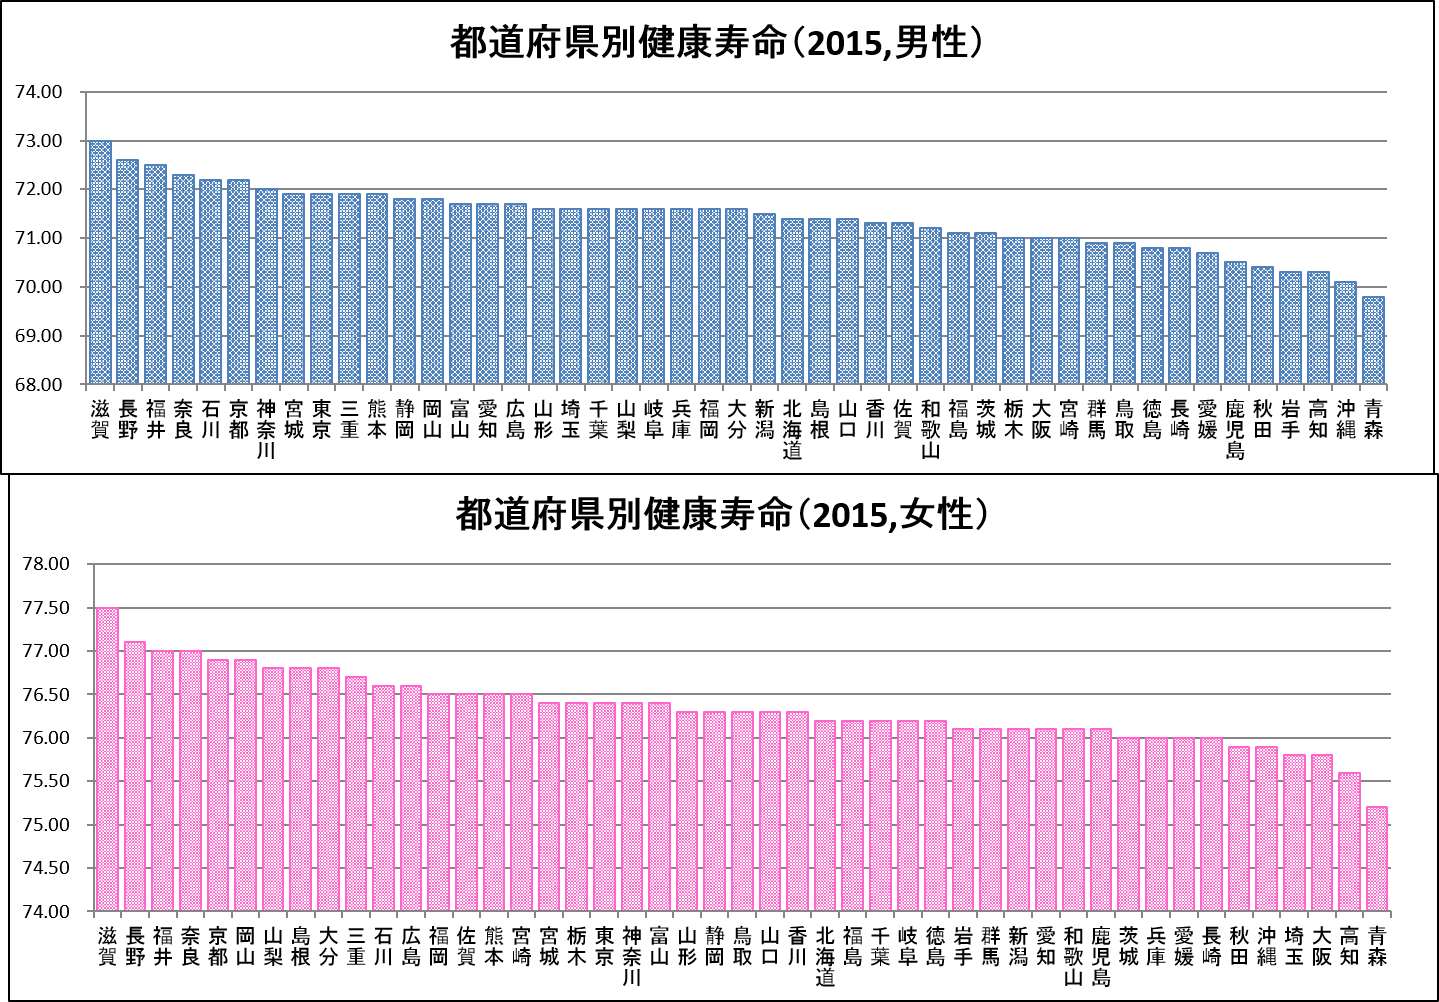
\includegraphics[ width=0.5\linewidth]{fig/fig11.png}
		% \put(-0.9,0.6){$\leftarrow$滋賀県 男性, 1位}
		% \put(-0.9,0.25){$\leftarrow$滋賀県 女性, 1位}
		\caption{都道府県別の健康寿命(2015年)}\label{fig11}
	\end{center}
\end{figure}

図\ref{fig11}は同研究のデータに基づき, 衛生科学センターより再編・加工し都道府県別の健康寿命を示した図である. 図から分かるように, 滋賀県は健康寿命においても, 全国1位を示しており, 寿命が長いだけではなく, 質の高い長生きしている現状がデータから見られた.

野村ら(2017)の研究で強調している内容は健康問題における地域格差問題であり, 各地域の疾病構造, 健康の位置づけに基づいて適切な「健康変換」をおこなう必要があると主張している. しかし, 健康格差の原因究明までにはまだ至らなかった. 従って, 滋賀県が健康な県である理由を示すことは, 全国の健康格差を縮めることに寄与すると考えられる.

%この研究の結果は滋賀県の現在の位置づけが健康格差の首位に位置づけら健康の地域
%同研究では, 健康寿命滋賀県の健康に関する報告は
%次は, 「世界の疾病負荷研究(Global Burden of Diseases, Injuries, and Risk Factor Study)」 の一環として,
%行った野村ら(Lancet, 2017)の最新研究の内容の一部を取り上げる.
%

\section{健康寿命3指標比較}
\begin{figure}[h!]
	\begin{center}
		%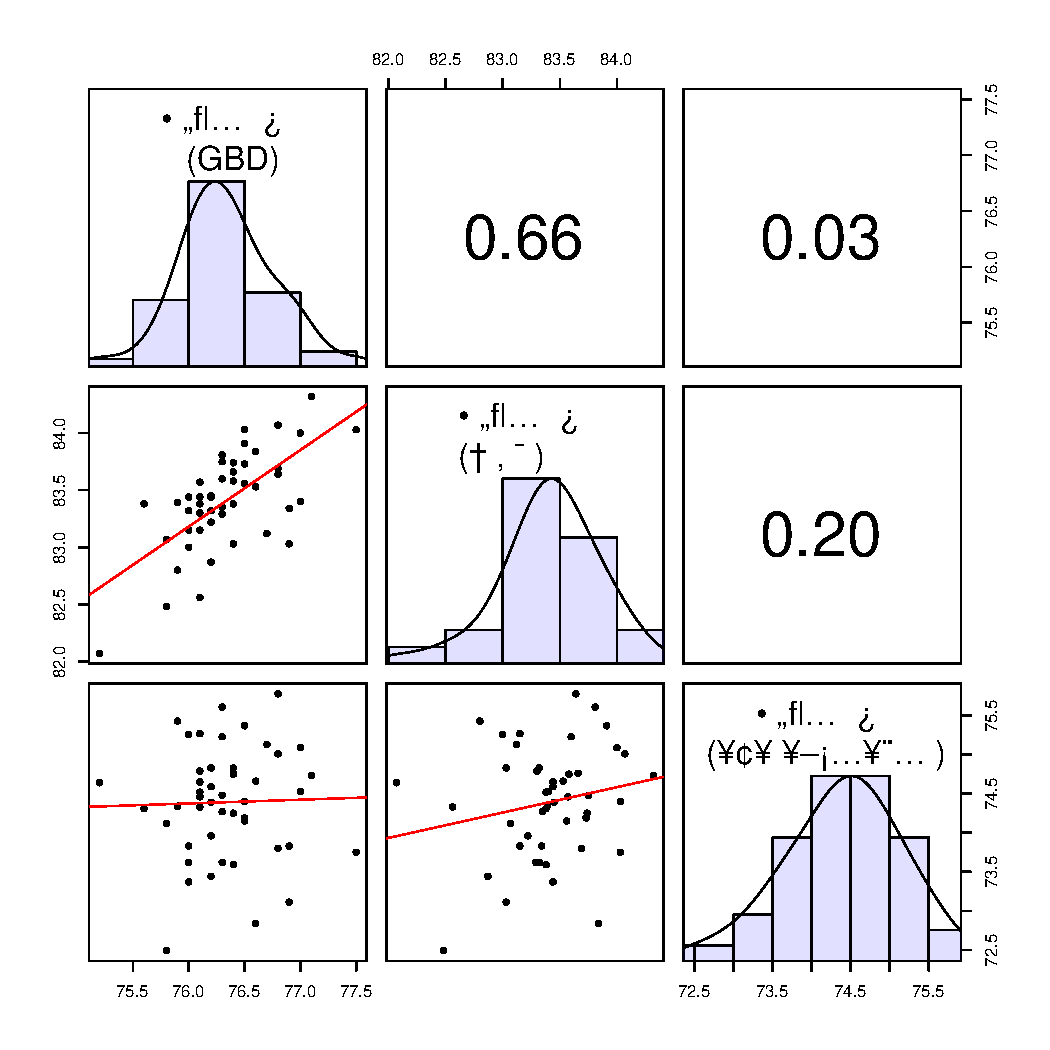
\includegraphics[ width=0.5\linewidth]{fig/3idxF.pdf}
		%     \put(-0.9,0.6){$\leftarrow$滋賀県 男性, 1位}
		%     \put(-0.9,0.25){$\leftarrow$滋賀県 女性, 1位}
		\caption{健康寿命3指標相関(女性)}
	\end{center}
\end{figure}

\begin{figure}[h!]
	\begin{center}
		%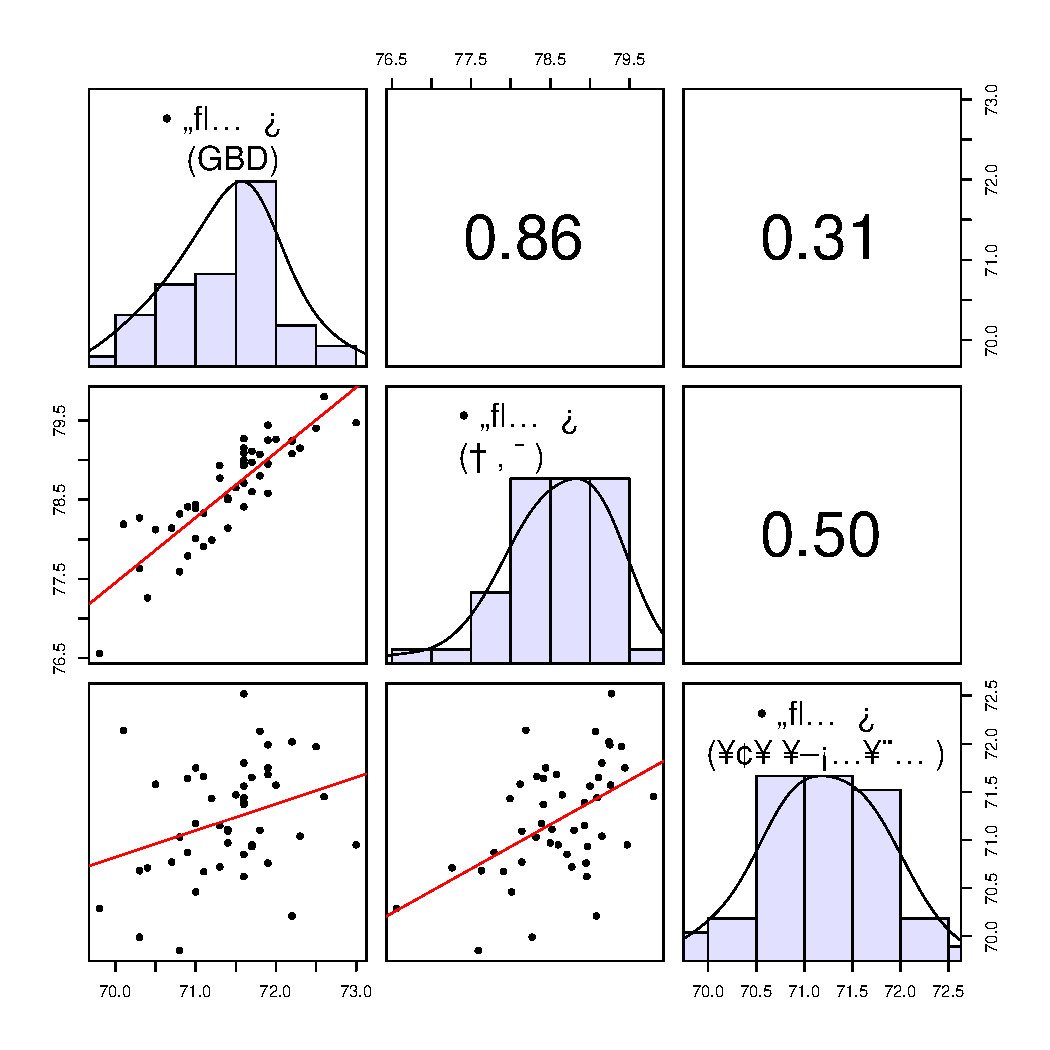
\includegraphics[ width=0.5\linewidth]{fig/3idxM.pdf}
		%     \put(-0.9,0.6){$\leftarrow$滋賀県 男性, 1位}
		%     \put(-0.9,0.25){$\leftarrow$滋賀県 女性, 1位}
		\caption{健康寿命3指標相関(男性)}
	\end{center}
\end{figure}



\begin{figure}[h!]
	\begin{center}
		%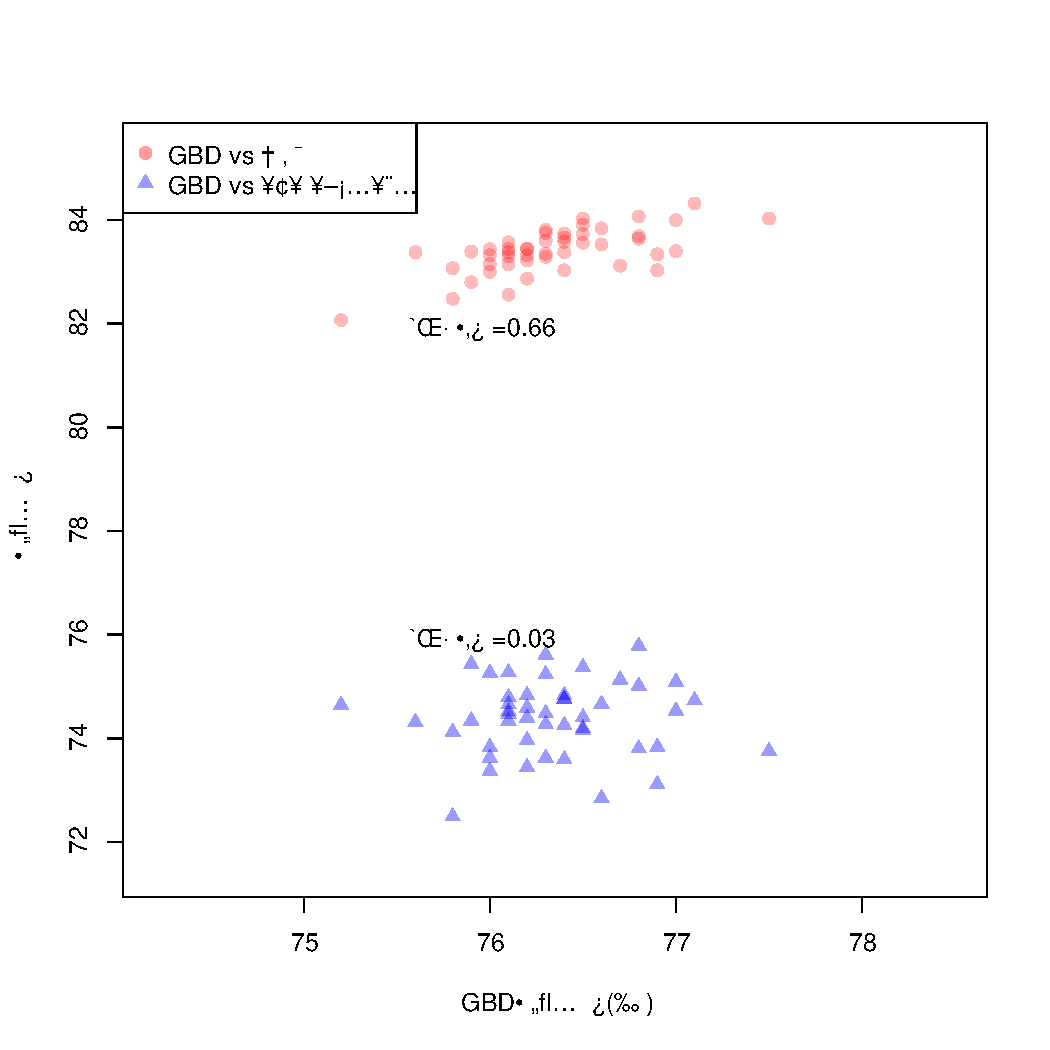
\includegraphics[ width=0.5\linewidth]{fig/HLcorrF.pdf}
		%     \put(-0.9,0.6){$\leftarrow$滋賀県 男性, 1位}
		%     \put(-0.9,0.25){$\leftarrow$滋賀県 女性, 1位}
		\caption{健康寿命3指標相関(女性)}
	\end{center}
\end{figure}



\begin{figure}[h!]
	\begin{center}
		%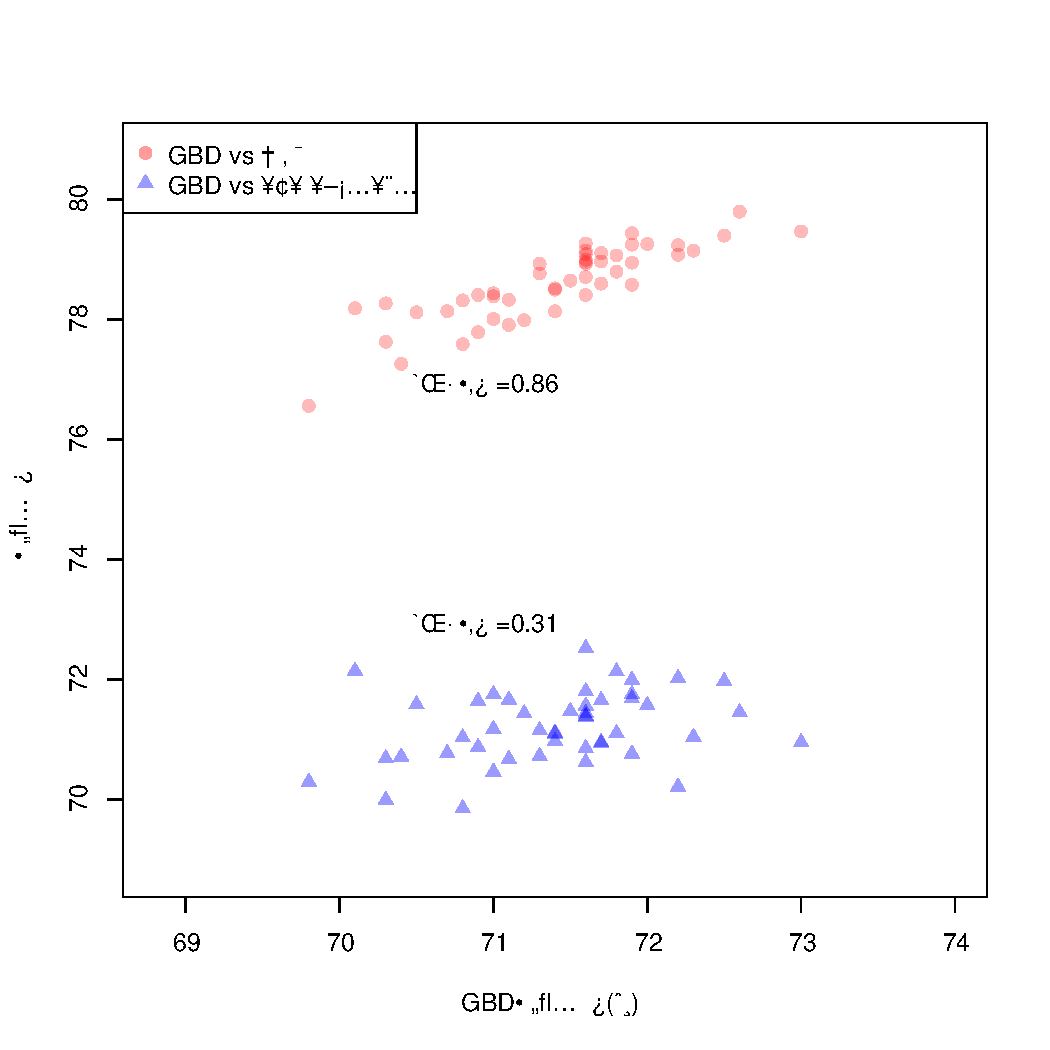
\includegraphics[ width=0.5\linewidth]{fig/HLcorrM.pdf}
		%     \put(-0.9,0.6){$\leftarrow$滋賀県 男性, 1位}
		%     \put(-0.9,0.25){$\leftarrow$滋賀県 女性, 1位}
		\caption{健康寿命3指標相関(男性)}
	\end{center}
\end{figure}

\begin{figure}[h!]
	\begin{center}
		%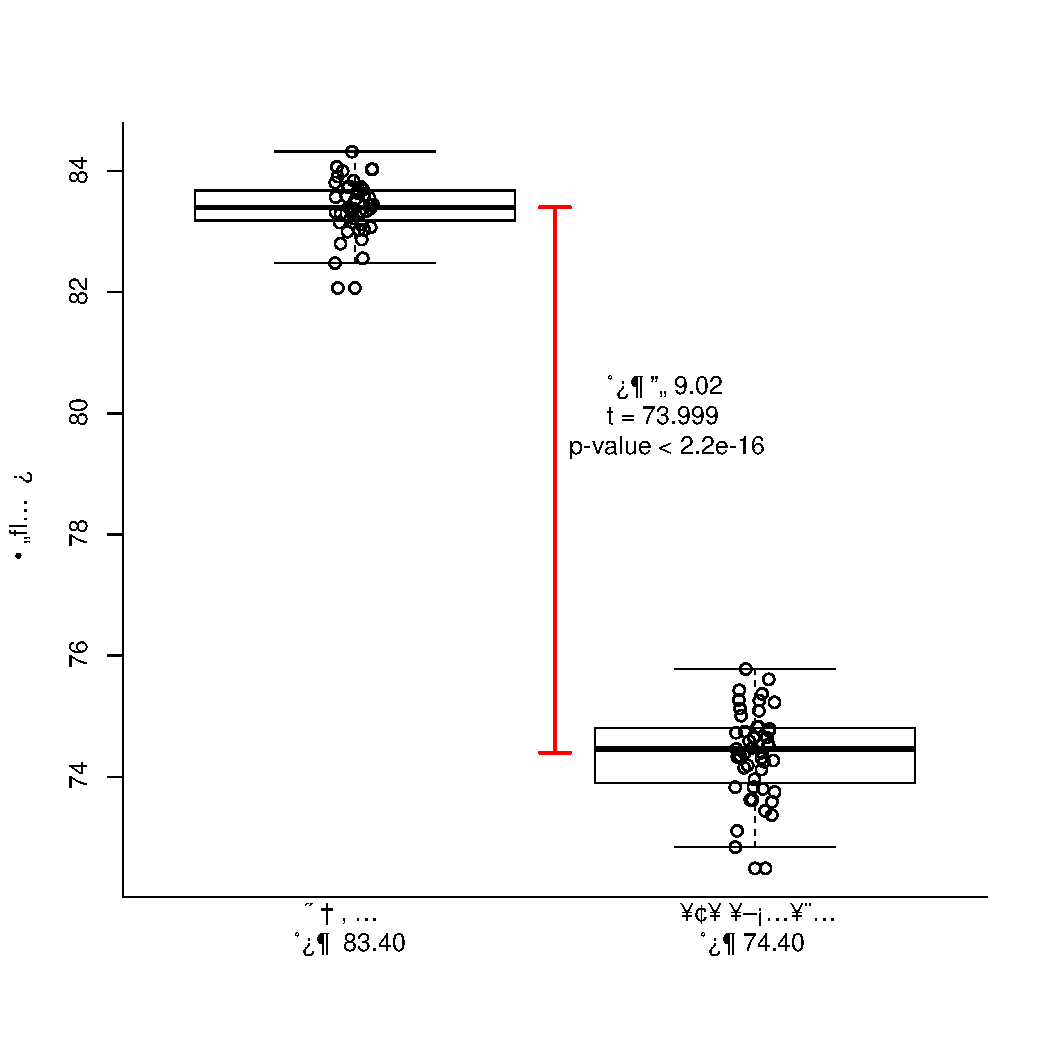
\includegraphics[ width=0.5\linewidth]{fig/ttestF.pdf}
		%     \put(-0.9,0.6){$\leftarrow$滋賀県 男性, 1位}
		%     \put(-0.9,0.25){$\leftarrow$滋賀県 女性, 1位}
		\caption{介護度式とアンケート式間健康寿命の平均差比較(女性)}
	\end{center}
\end{figure}

\begin{figure}[h!]
	\begin{center}
		%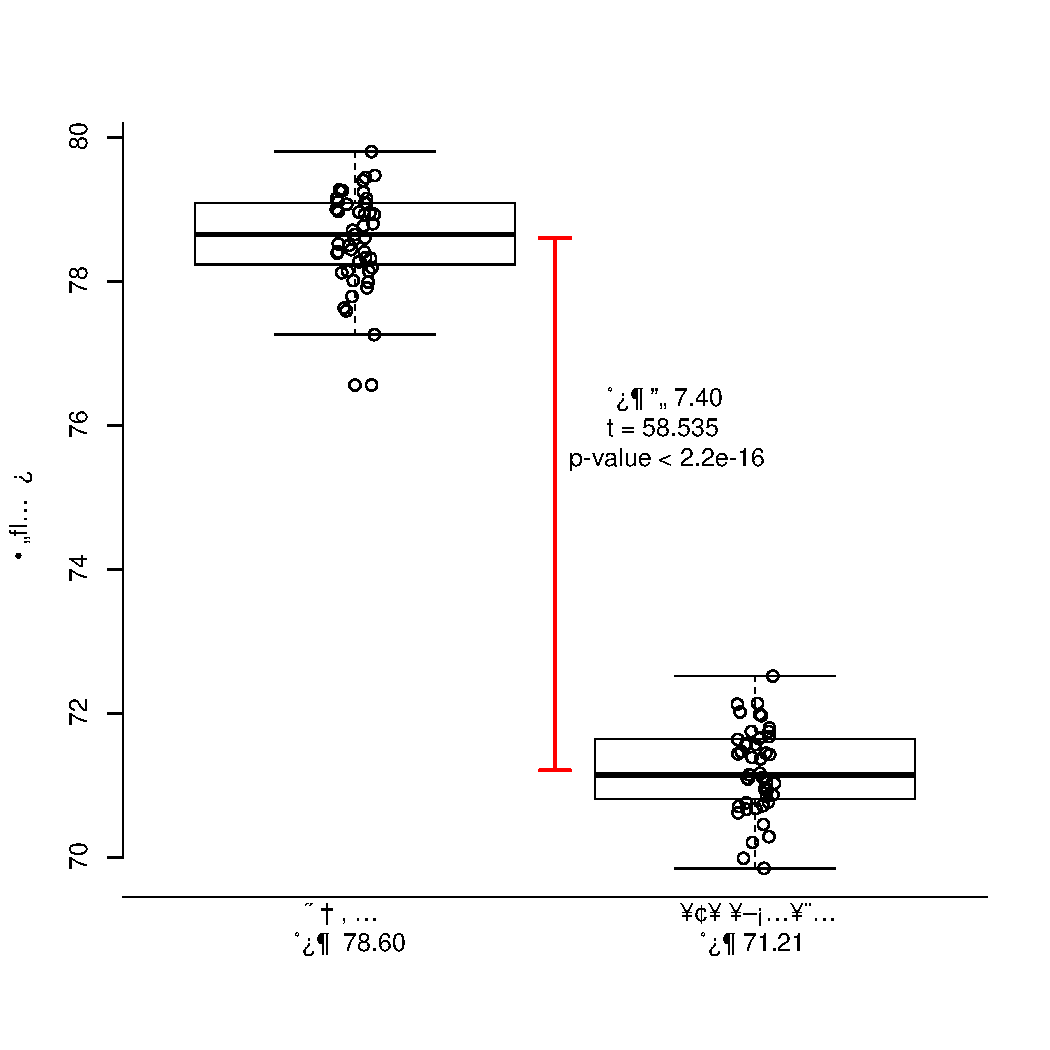
\includegraphics[ width=0.5\linewidth]{fig/ttestM.pdf}
		%     \put(-0.9,0.6){$\leftarrow$滋賀県 男性, 1位}
		%     \put(-0.9,0.25){$\leftarrow$滋賀県 女性, 1位}
		\caption{介護度式とアンケート式間健康寿命の平均差比較(男性)}
	\end{center}
\end{figure}




%------------------------------------------------------------
\chapter{健康寿命と関連のある要因探索}
%------------------------------------------------------------

滋賀県民の健康寿命の延伸を図ることに当たって, 科学的根拠に基づいた効果的な取り組みを進める必要がある. そのため, まず, 健康寿命に影響を与える要因を探索することが第一歩となる.
本章では, 都道府県別の健康寿命と健康および社会要因と関連のするデータを利用し健康寿命との相関分析と単回帰分析を行った.
%その結果から男女別に効果的な施策を提案することを目的とした.

\section{相関分析に用いる変数}
都道府県別の健康寿命データは2013年の都道府県別の「平均自立期間」\footnote{「平均自立期間」は「要介護2以上」を「不健康」として定義し手算出する. 「厚生労働科学研究費補助金による健康寿命における将来予測と生活習慣病対策の費用対効果に関する研究班報告書」}を採用した. 「平均自立期間」との相関分析のため対になる変数においては, 通常, 健康と直接に関係があると見られる「健康変数」と間接的に影響を与えうる「社会変数」を選び都道府県別に相関分析を行うことにする.

健康変数はさらに, 健康の指標を直接に示す変数と健康向上にむけての生活習慣と関連がある健康行動変数の2種類に分けた. 詳細は下記の通りである.
\begin{itemize} \setlength{\itemsep}{-0.5mm} \setlength{\parskip}{-0.5mm}
	\item 健康指標変数(health index)
	      \begin{itemize} \setlength{\itemsep}{-0.5mm} \setlength{\parskip}{-0.5mm}
		      \item 	肥満度(BMI)
		      \item 	野菜摂取量
		      \item 	食塩摂取量
	      \end{itemize}

	\item 健康行動変数(health behavior)
	      \begin{itemize} \setlength{\itemsep}{-0.5mm} \setlength{\parskip}{-0.5mm}
		      \item 	平均歩数
		      \item 	喫煙率
		      \item 	1人当たりアルコール消費量
	      \end{itemize}
\end{itemize}

社会変数も健康変数と同じく二つに分けて, ある社会の健全性を測る社会指標変数と個人レベルで行っている社会行動変数の2種類で構成した. 社会変数の詳細は下記の通りである.

\begin{itemize} \setlength{\itemsep}{-0.5mm} \setlength{\parskip}{-0.5mm}
	\item 社会指標変数(social index)
	      \begin{itemize} \setlength{\itemsep}{-0.5mm} \setlength{\parskip}{-0.5mm}
		      \item 	GINI係数
		      \item 	住みやすさ %http://toyokeizai.net/articles/-/177578?page=2
	      \end{itemize}
	\item 社会行動変数(social behavior)
	      \begin{itemize} \setlength{\itemsep}{-0.5mm} \setlength{\parskip}{-0.5mm}
		      \item 	ボランティア参加率
		      \item 	余暇でスポーツをしている割合
		      \item 	趣味・娯楽を持っている割合
		      \item 	学習・自己啓発をしている割合
	      \end{itemize}
\end{itemize}

\subsection{データの出典}
都道府県別の上記のデータは
総務省の「2011年社会生活基本調査」によりボランティアをしている割合, 余暇でスポーツをしている割合, 趣味・娯楽を持っている割合, 学習・自己啓発をしている割合,
厚生労働省の「2012年国民健康・栄養調査」により肥満度, 野菜摂取量, 食塩摂取量, 平均歩数, 喫煙率,
2013年国税庁の国税庁統計情報資料より算出された「都道府県別統計ランキングでみる県民性」
\footnote{\url{http://todo-ran.com/t/kiji/14569}より引用}より一人平均アルコール消費量データを採用した.
住みさ変数は東洋経済新聞の発表により, GINI係数は総務省のHP\footnote{\url{http://www.e-stat.go.jp/SG1/estat/List.do?bid=000001075200&cycode=0}}により手入した.

%アルコールは
%
%
%
%ジニ係数は
%http://www.e-stat.go.jp/SG1/estat/List.do?bid=000001075200&cycode=0
%
%です
%無相関分析
%http://cse.naro.affrc.go.jp/takezawa/r-tips/r/67.html

\section{相関分析結果}

%\begin{table*}
% \caption{都道府県別の男女別健康寿命と生活習慣との相関係数}
%\begin{tabular}{c||cccccc}
%\hline
%健康要因 & 健康指標 &  &  & 健康行動 &  &  \\
% & BMI & 野菜 & 食塩 & 歩数 & 喫煙率 & アルコール \\\hline
%男 & -0.35 & 0.11 & 0.09 & 0.21 & -0.3 & -0.38 \\
%女 & -0.17 & 0.13 & 0.1 & 0.23 & - & - \\\hline
%社会要因 & 社会指標 &  & 社会指標 &  &  &  \\
% & ジニ係数 & 住みやすさ & ボランティア & スポーツ & 趣味娯楽 & 学習 \\\hline
%男 & 0.38 & 0.65 & 0.09 & 0.66 & 0.59 & 0.58 \\
%女 & 0.3 & 0.91 & 0.56 & 0.27 & 0.13 & 0.22 \\
%\hline
%\end{tabular}
%\end{table*}
%
\begin{table*}
	\centering
	\caption{都道府県別の男女別健康寿命と健康要因との相関係数}
	\begin{tabular}{c||ccc|ccc}
		\hline
		健康要因 & 健康指標   &      &      & 健康行動 &           &            \\
		         & BMI        & 野菜 & 食塩 & 歩数     & 喫煙率    & アルコール \\\hline
		男       & \tr{-0.35} & 0.11 & 0.09 & 0.21     & \tr{-0.3} & \tr{-0.38} \\
		女       & -0.17      & 0.13 & 0.1  & 0.23     & -         & -          \\\hline
	\end{tabular}
\end{table*}


\begin{table*}
	\centering
	\caption{都道府県別の男女別健康寿命と社会要因との相関係数}
	\begin{tabular}{c||cc|cccc}
		\hline
		社会要因 & 社会指標   &            & 社会行動     &           &           &           \\
		         & ジニ係数   & 住みやすさ & ボランティア & スポーツ  & 趣味娯楽  & 学習      \\\hline
		男       & \tr{-0.62} & \tr{0.81}  & 0.09         & \tr{0.66} & \tr{0.59} & \tr{0.58} \\
		女       & \tr{-0.55} & \tr{0.95}  & \tr{0.56}    & 0.27      & 0.13      & 0.22      \\
		\hline
	\end{tabular}
\end{table*}




%\begin{figure}[h!]
%\begin{center}
%    %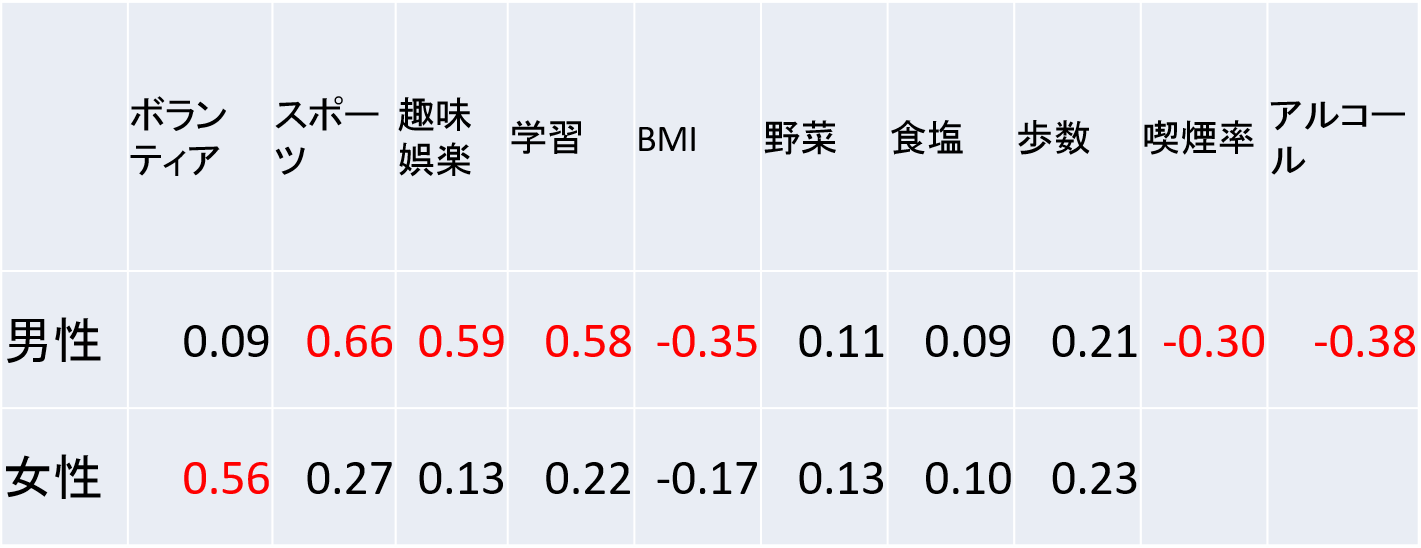
\includegraphics[ width=0.5\linewidth]{fig/fig16.png}
%%     \put(-0.9,0.6){$\leftarrow$滋賀県 男性, 1位}
%%     \put(-0.9,0.25){$\leftarrow$滋賀県 女性, 1位}
%   \caption{都道府県別の男女別健康寿命と生活習慣との相関係数}
%\end{center}
%\end{figure}
標本のサイズが$n=47$
(47都道府県), 有意水準5\%の下で, 標本相関係数 $r$の絶対値が0.29以上であれば, 有意な相関があると言える.\footnote{母相関係数における「$H_0 ~: ~\rho=0$」の仮説検定統計量
	$|T|=\left|\frac{r\sqrt{n-2}}{\sqrt{1-r^2}}\right|
		\ge t_{0.025, 45}=2.014$により算出すると$|r|>0.48$以上.
	有意水準10\%の下では
	$|r|>0.45$.
}
%http://www.ipc.shimane-u.ac.jp/food/kobayasi/biometry12_2010.html
上記の表は健康寿命とそれぞれの変数との相関係数の結果である.
健康寿命の延伸に繋がる可能性のある生活習慣対策としては
男性では, スポーツ習慣の普及, 趣味・娯楽の普及, 肥満対策, 禁煙対策, 節酒対策が,
女性ではボランティアへの参加促進対策が重要であることを示唆している.
\section{単回帰分析-健康変数}
\subsection{健康指標変数}
\begin{figure}[h!]
	\begin{center}
		%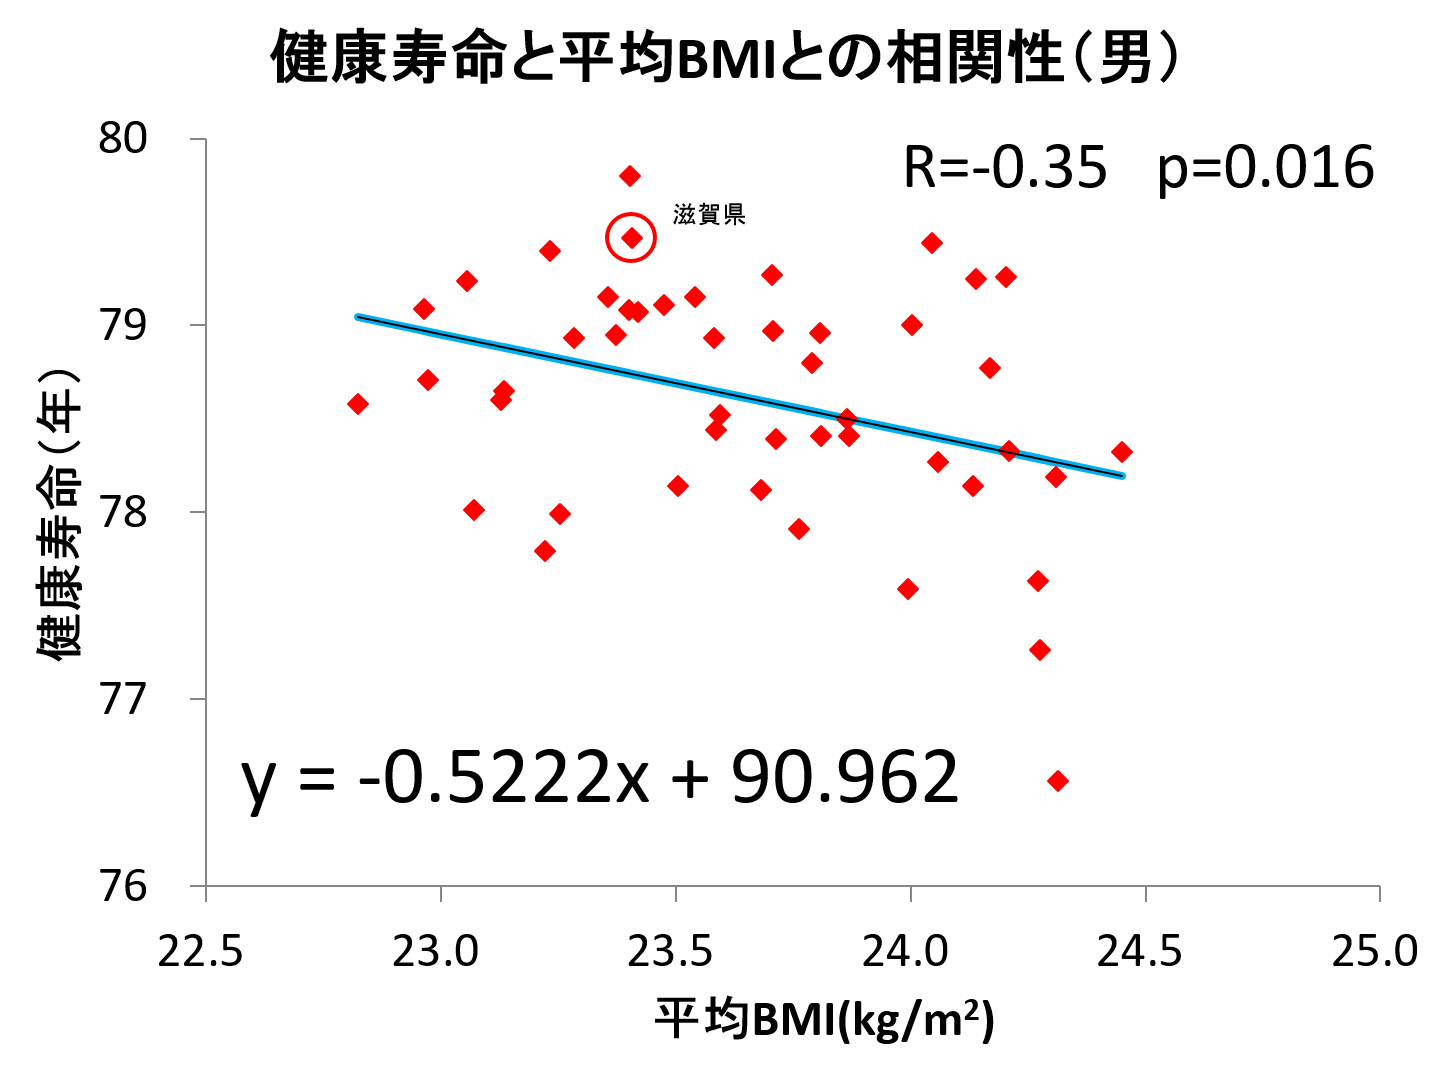
\includegraphics[ width=0.5\linewidth]{fig/fig18.png}
		\caption{BMI(男)}\end{center}
\end{figure}


\subsection{健康行動変数}
\begin{figure}[h!]
	\begin{center}
		%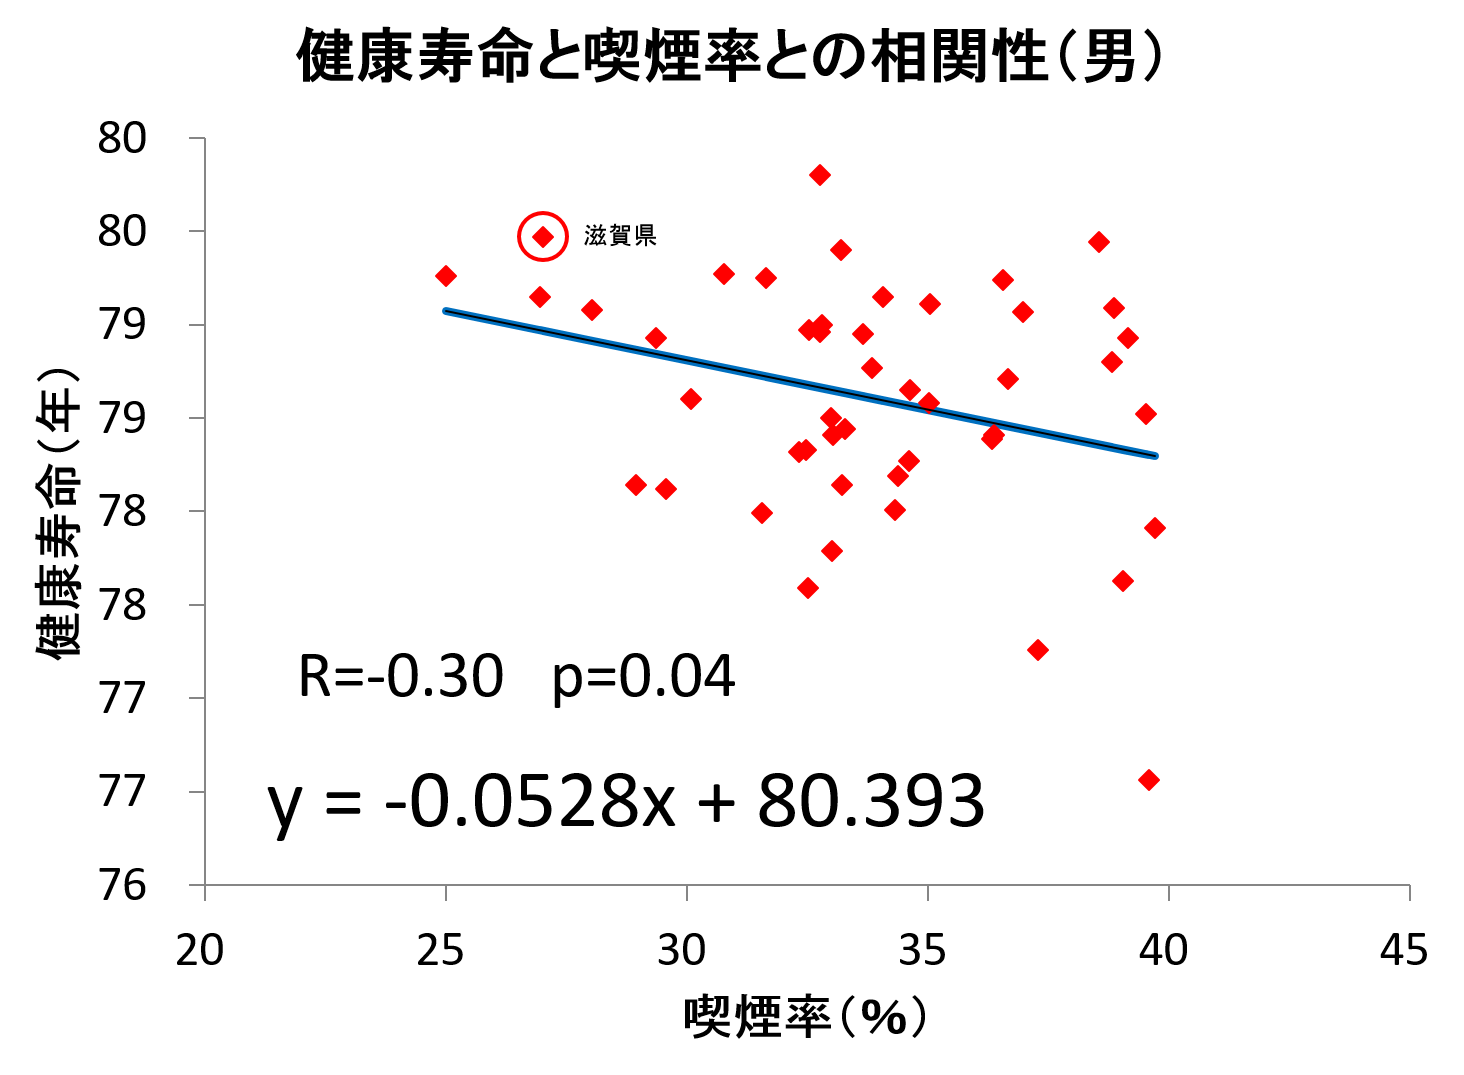
\includegraphics[ width=0.49\linewidth]{fig/fig19.png}
		%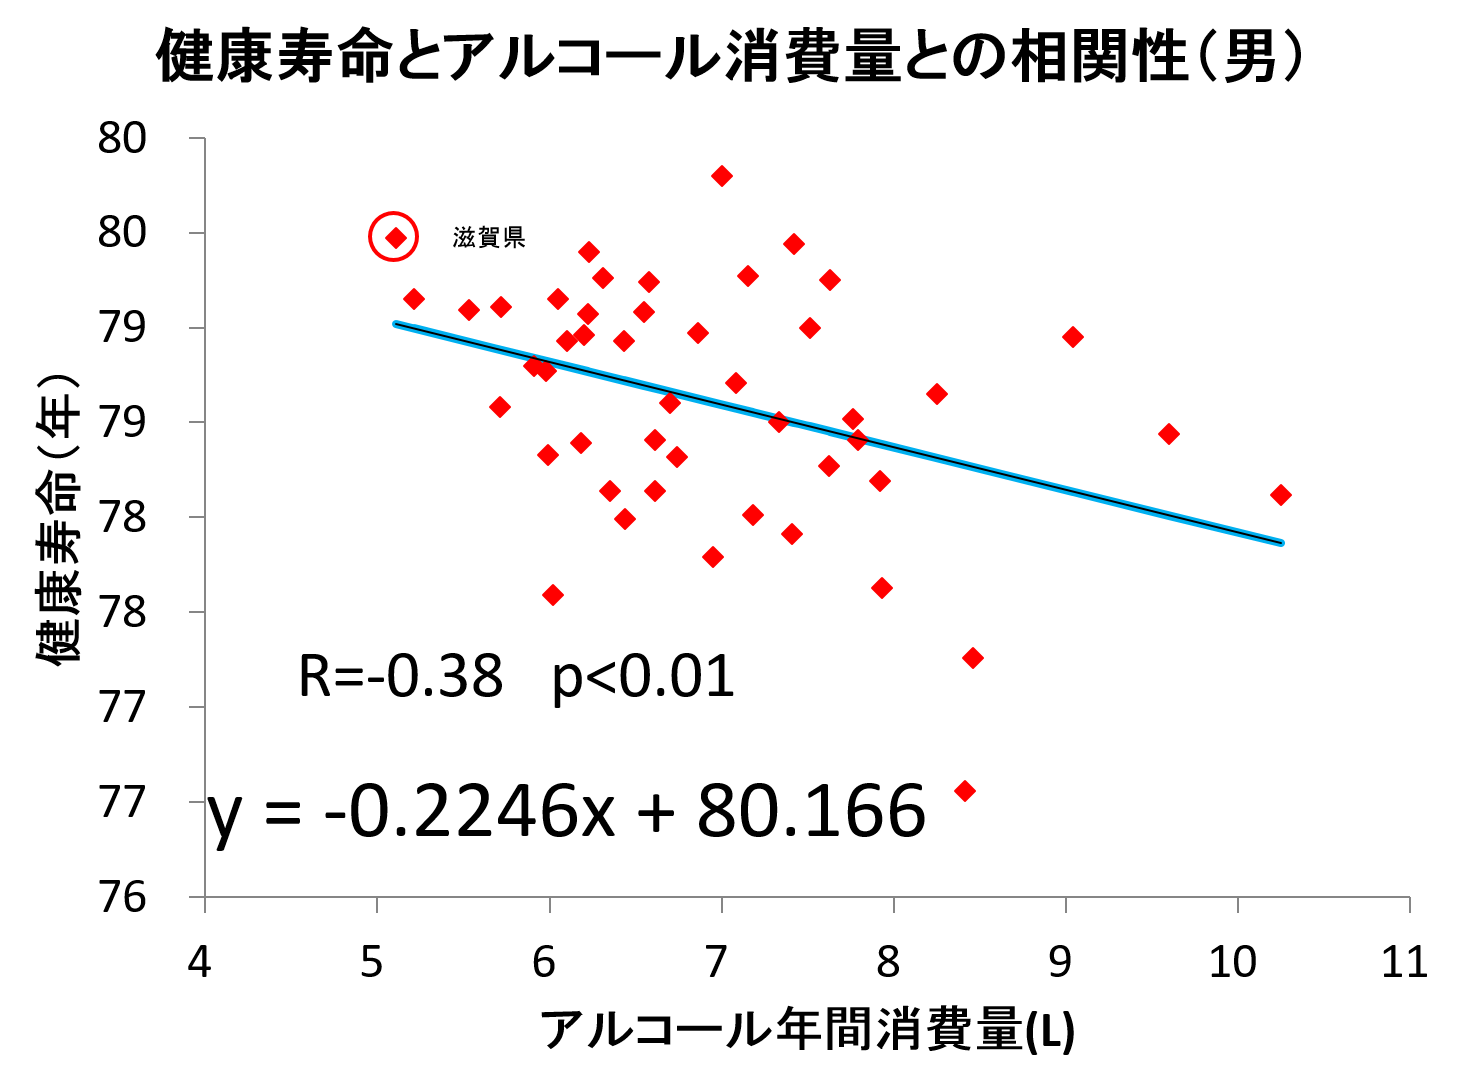
\includegraphics[ width=0.49\linewidth]{fig/fig20.png}
		\caption{喫煙率(左)とアルコール消費量(右), 男}\end{center}
\end{figure}




\section{単回帰分析ー社会変数}
\subsection{社会指標変数}
\begin{figure}[H]
	\begin{center}
		%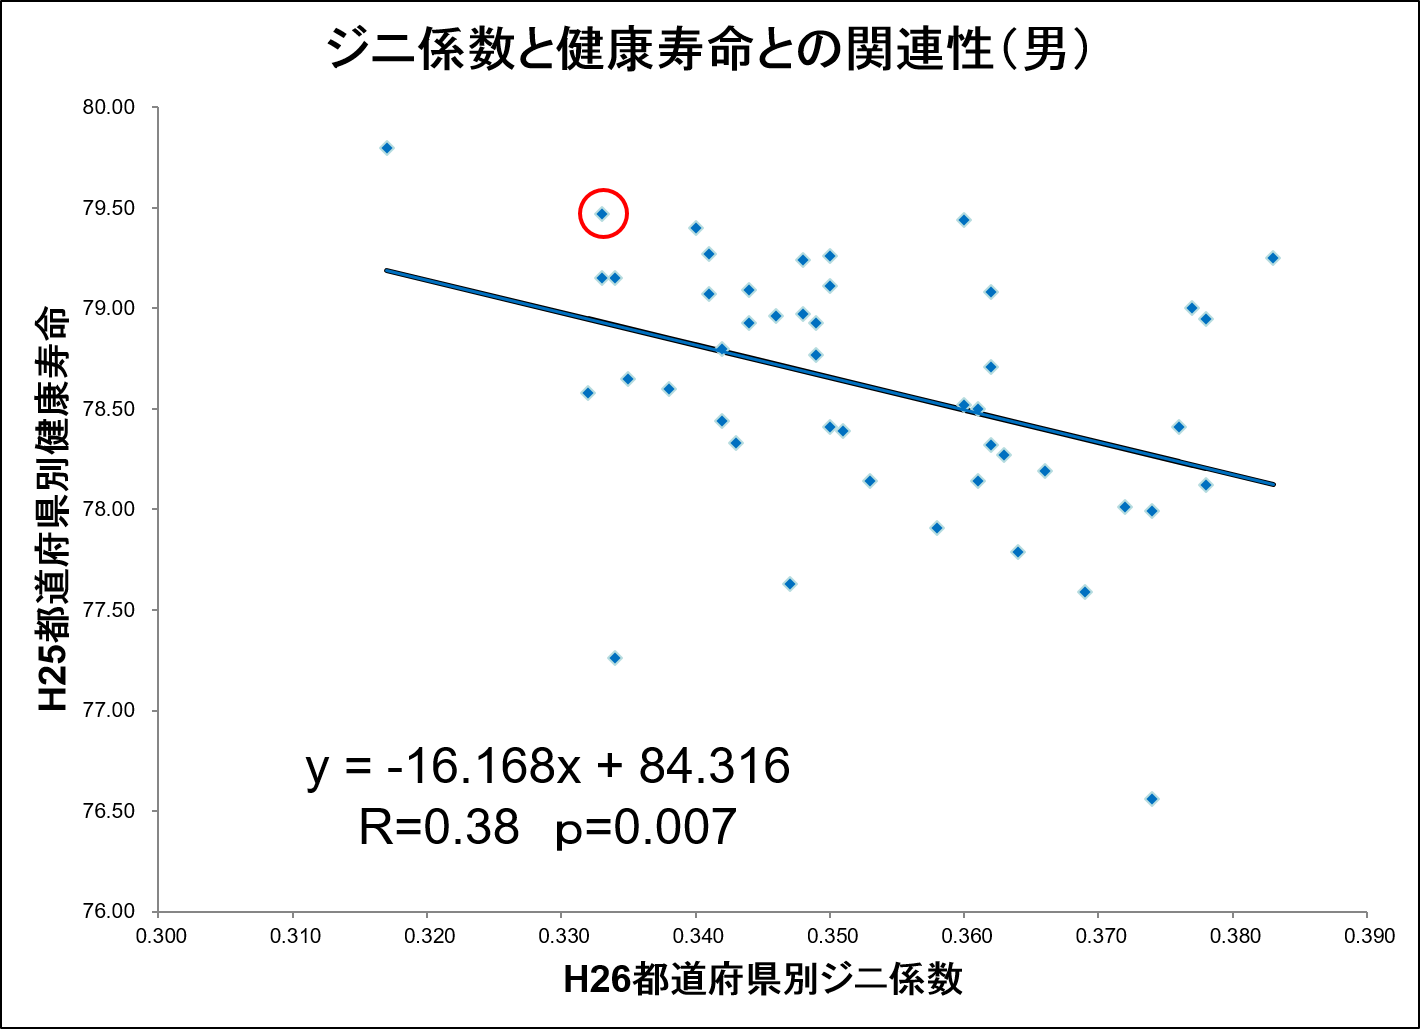
\includegraphics[ width=0.49\linewidth]{fig/fig22.png}
		%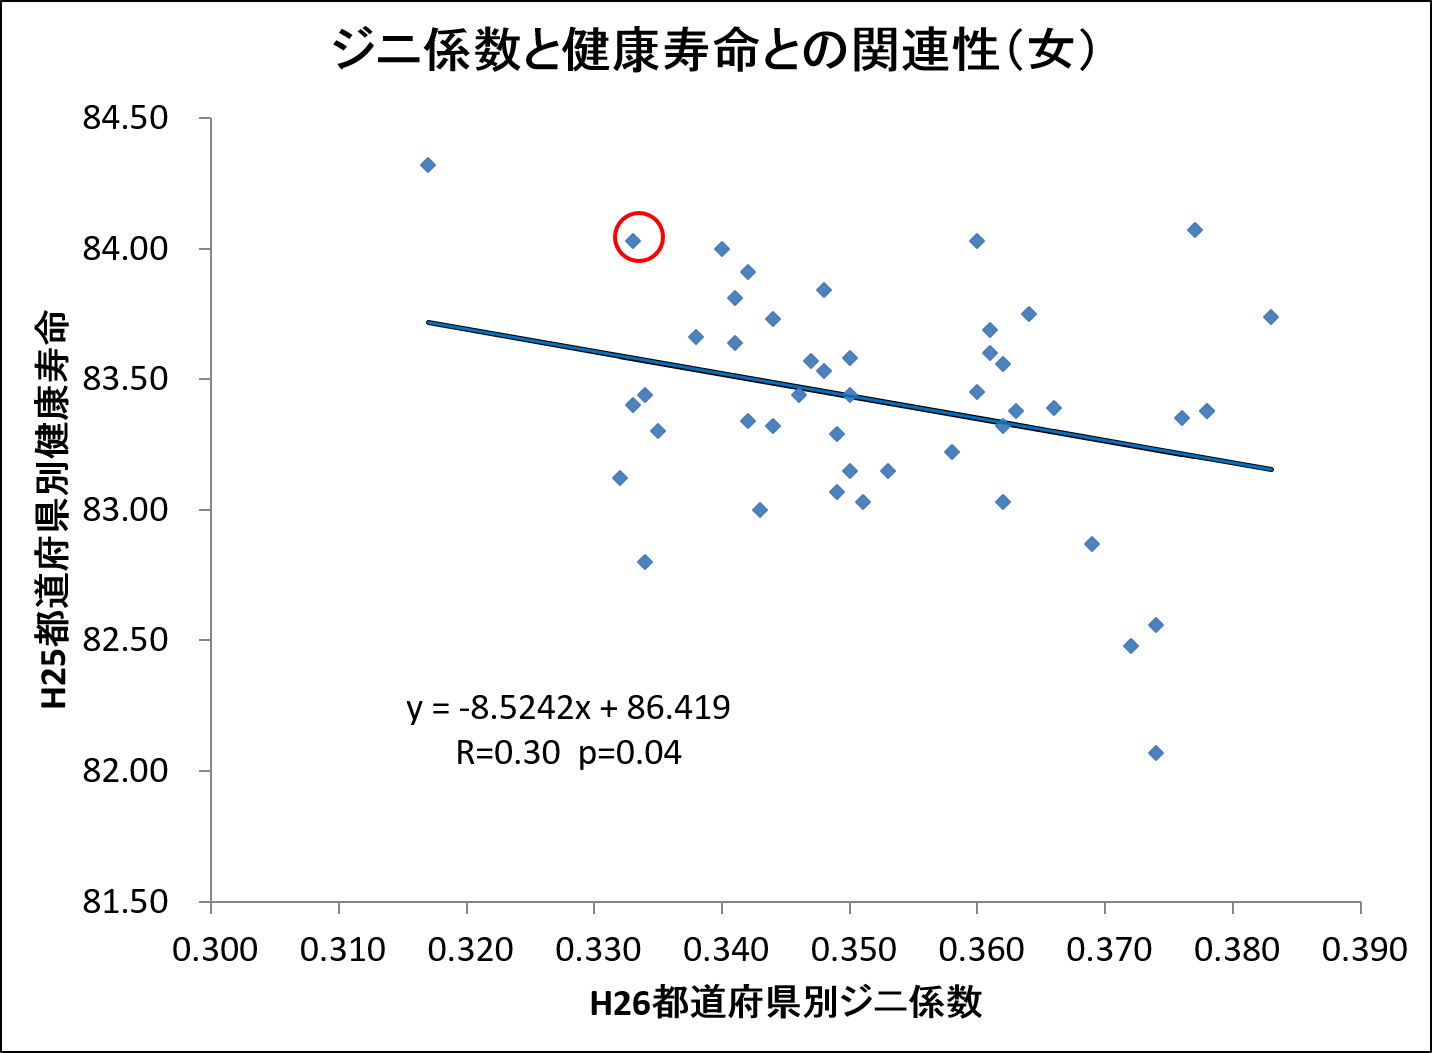
\includegraphics[ width=0.49\linewidth]{fig/fig23.png}
		%     \put(-0.9,0.6){$\leftarrow$滋賀県 男性, 1位}
		%     \put(-0.9,0.25){$\leftarrow$滋賀県 女性, 1位}
		\caption{ジニ係数(男, 女)}
	\end{center}
\end{figure}

\begin{figure}[h!]
	\begin{center}
		%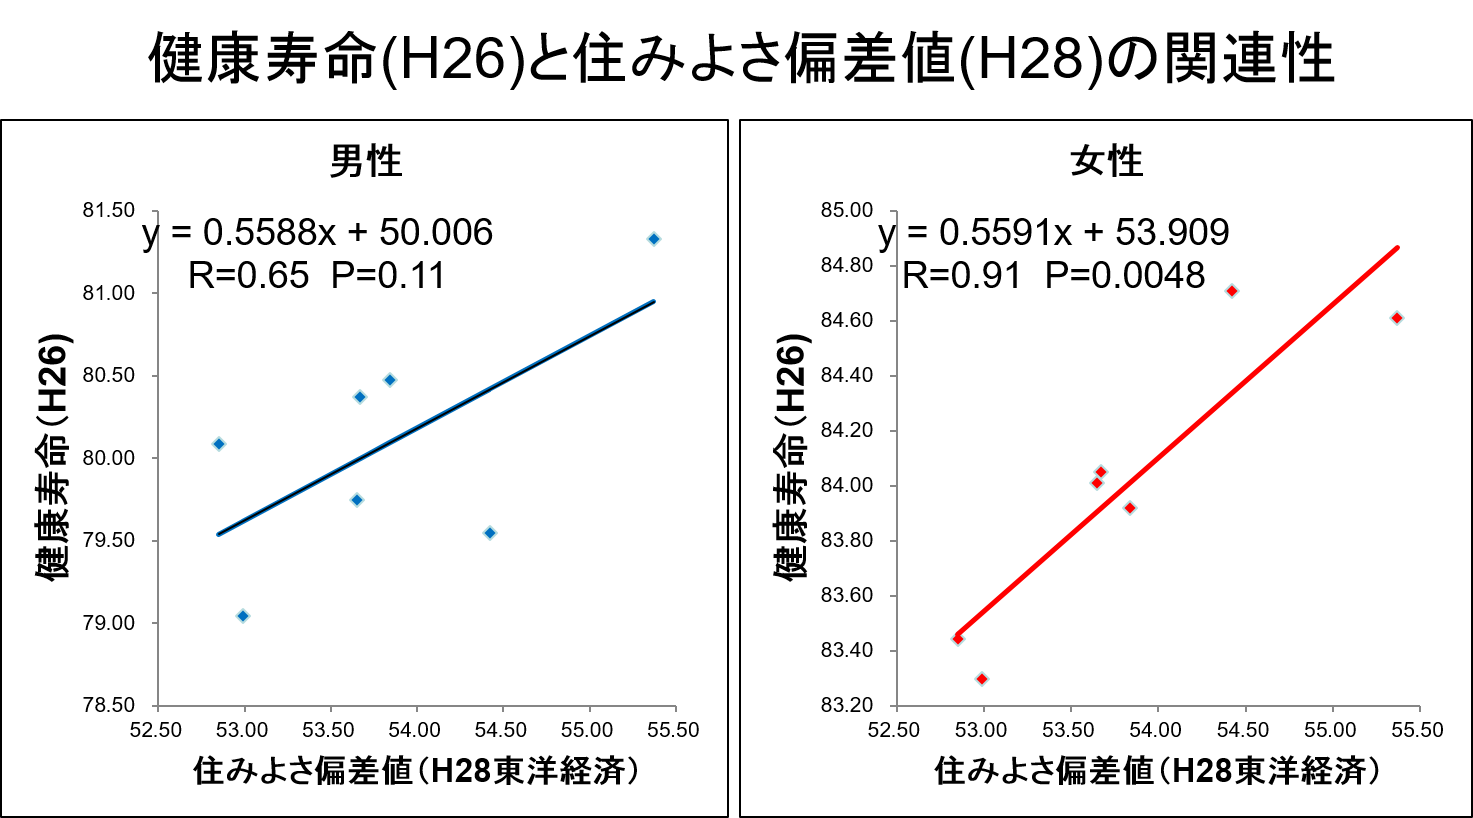
\includegraphics[ width=0.5\linewidth]{fig/fig24.png}
		%     \put(-0.9,0.6){$\leftarrow$滋賀県 男性, 1位}
		%     \put(-0.9,0.25){$\leftarrow$滋賀県 女性, 1位}
		\caption{住み良さ}
	\end{center}
\end{figure}


\subsection{社会行動変数}

\begin{figure}[h!]
	\begin{center}
		%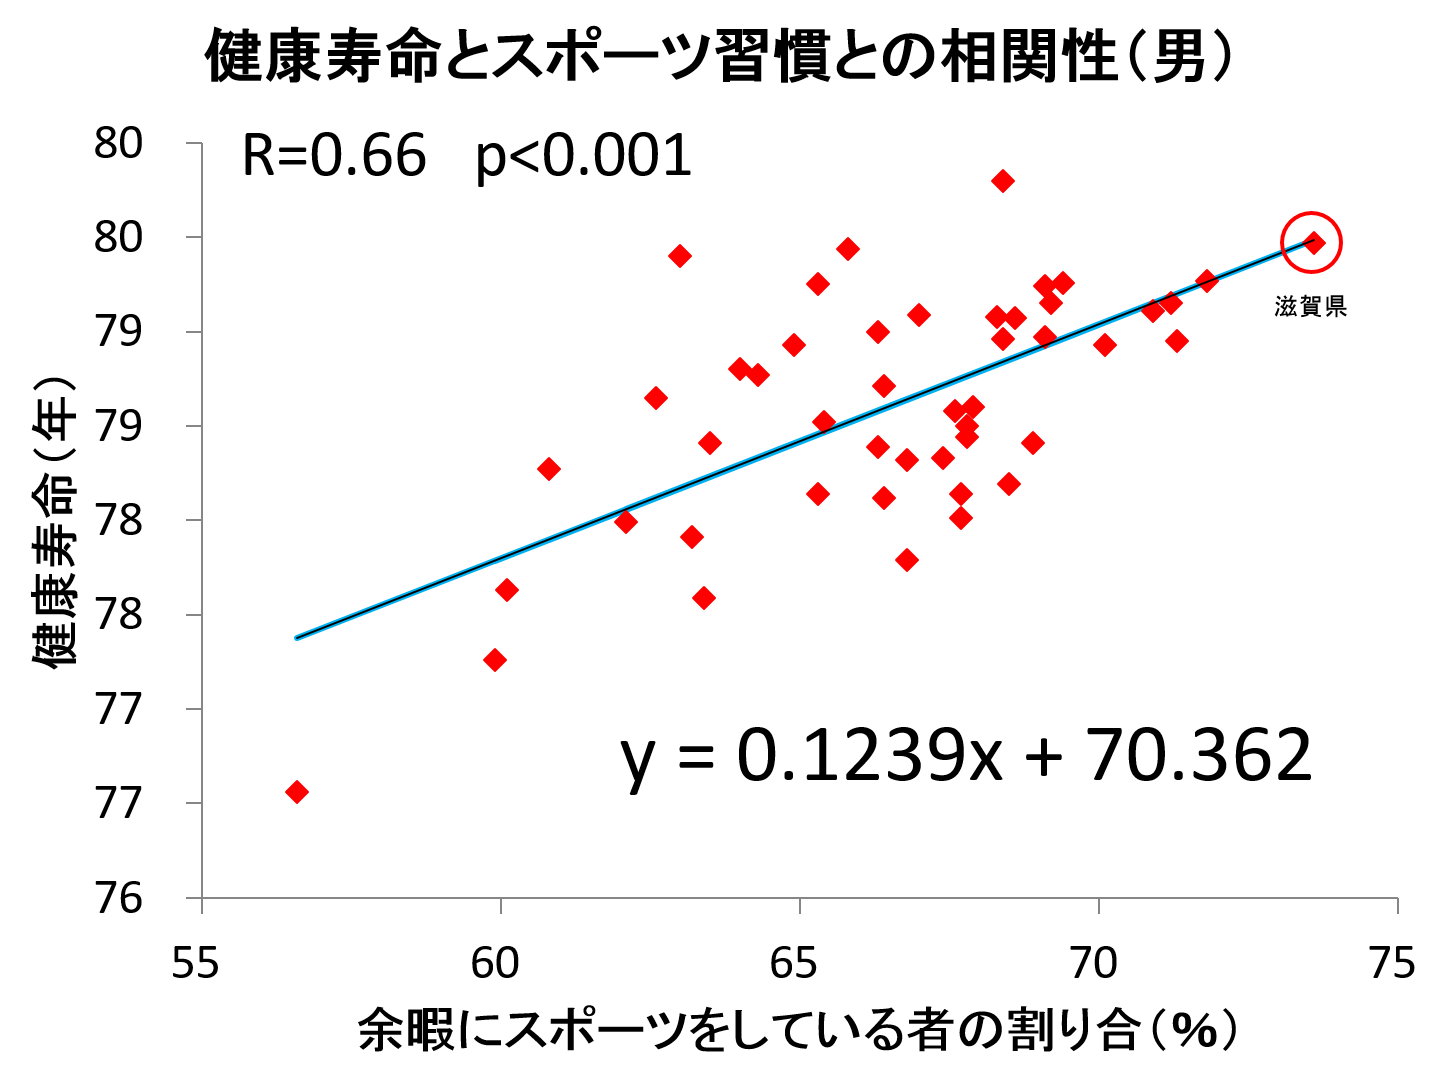
\includegraphics[ width=0.49\linewidth]{fig/fig17.png}
		%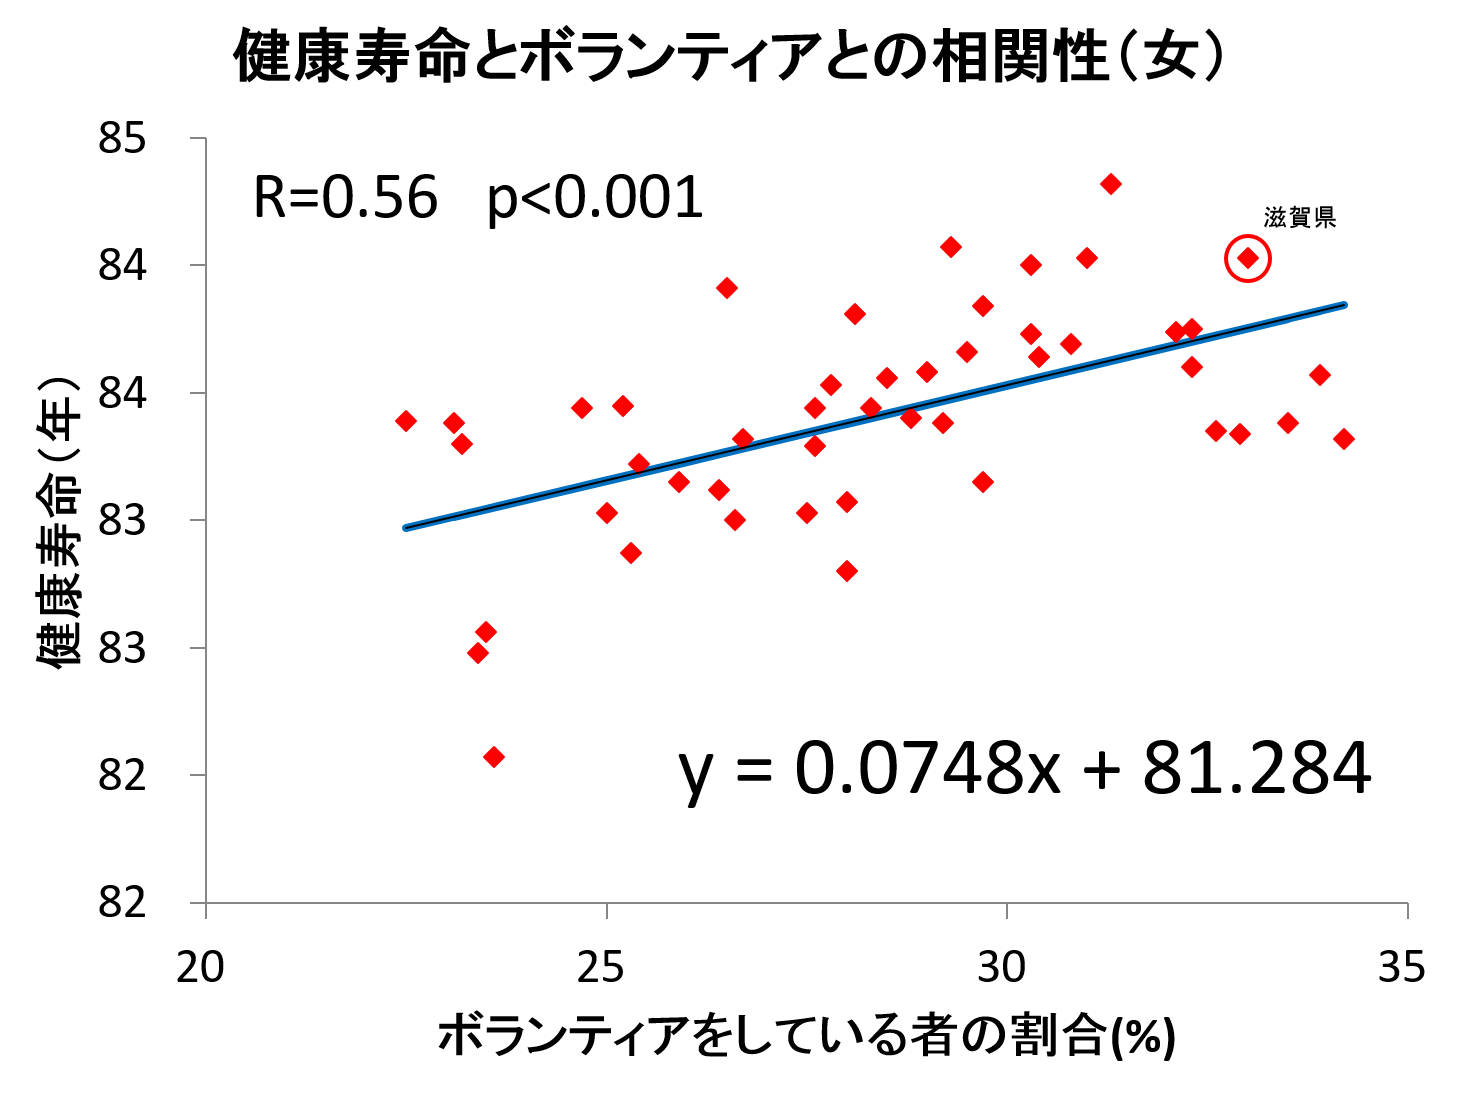
\includegraphics[ width=0.49\linewidth]{fig/fig21.png}
		\caption{スポーツ(男)とボランティア活動(女)}\label{fig17}
	\end{center}
\end{figure}



%ローレンツ曲線が右下にあるほど格差が大きい.
%ジニ係数が大きいほど格差が大きい.
%
%https://mathwords.net/ginikeisu
%http://www.pref.toyama.jp/sections/1015/ecm/back/2005apr/shihyo/

%------------------------------------------------------------
\chapter{統計解析概要}
%------------------------------------------------------------
\section{データ}
表\ref{variable}に本研究に用いるデータの構成と変数一覧を示す。

\begin{table*}[h!]
	\centering
	\caption{変数一覧}
	\label{variable}
	\begin{tabular}{ll}
		\hline
		変数区分                 & 内容                                       \\ \hline
		目的変数                 & 健康寿命、GBD 2015より算出                 \\
		                         & 健康寿命、2013年国民保健の要介護度より算出 \\
		                         & 健康寿命3群(健康寿命上・中・下群)          \\ \hline
		説明変数(社会・生活変数) & 60代の自殺率の単位%、5年間合計            \\
		                         & 70代の自殺率の単位%、5年間合計            \\
		                         & 財政力指数                                 \\
		                         & 1人当たり医療費支出 (千円)                 \\
		                         & 1人当たり歯科医療費支出(円)                \\
		                         & BMI                                        \\
		                         & 野菜摂取率                                 \\
		                         & 塩分摂取量                                 \\
		                         & 徒歩数                                     \\
		                         & 喫煙                                       \\
		                         & 毎日お酒を飲んいる割合                     \\
		                         & 学習・自己啓発・訓練をしている割合         \\
		                         & ボランティア活動をしている割合             \\
		                         & スポーツをしている割合                     \\
		                         & 趣味を持っている割合                       \\
		                         & 旅行をしている割合                         \\
		                         & Gini係数(2014年)                           \\
		                         & 完全失業率                                 \\ \hline
		説明変数(健康変数)       & 疾患関連169変数 (GBDデータ)                \\
		                         & う蝕、歯周病、喪失歯関連110変数(NDBデータ) \\
		\hline
	\end{tabular}
\end{table*}

\section{相関による説明変数選択}
\begin{itemize} \setlength{\itemsep}{-0.5mm} \setlength{\parskip}{-0.5mm}
	\item 基本属性はそのまま利用
	\item 疾患系変数は相関が見られた変数のみ利用
	\item Pearson,Spearman 相関が0.01以下の示した項目のみ採用
	      \begin{itemize}
		      \item 疾患変数 164疾患の内134項目選択
		      \item 歯科関連変数は相関が見つからず。
	      \end{itemize}
\end{itemize}


\section{クラスター分析}
\begin{itemize} \setlength{\itemsep}{-0.5mm} \setlength{\parskip}{-0.5mm}
	\item 47都道府県の変数属性による類似度の可視化
\end{itemize}


\section{主成分分析}
\begin{itemize} \setlength{\itemsep}{-0.5mm} \setlength{\parskip}{-0.5mm}
	\item 疾患データを利用し主成分分析
	      \begin{itemize} \setlength{\itemsep}{-0.5mm} \setlength{\parskip}{-0.5mm}
		      \item biplot
		      \item 疾患変数を3〜4程度絞る
	      \end{itemize}
\end{itemize}


\section{対応分析}
\begin{itemize} \setlength{\itemsep}{-0.5mm} \setlength{\parskip}{-0.5mm}
	\item 疾患データを利用し疾患と都道府県間biplot 作成
\end{itemize}

\section{分類分析}
\begin{itemize} \setlength{\itemsep}{-0.5mm} \setlength{\parskip}{-0.5mm}
	\item 健康寿命に基づき、47都道府県を3つ(あるいは2つ)のグループに分けて、分類解析を行う。
	      \begin{itemize} \setlength{\itemsep}{-0.5mm} \setlength{\parskip}{-0.5mm}
		      \item SVM, Random forest, Kernel PCA など...
	      \end{itemize}

\end{itemize}


\section{回帰分析,logistic回帰}
\begin{itemize}
	\item 目的: 47都道府県別健康寿命($Y$) に影響を与える説明変数($X$)の特定やその影響の程度を統計解析の結果から示す。

	\item モデルのイメージ
	      \begin{itemize}
		      \item $Y$は健康寿命, $X$は都道府県別のデータ
		            $$ Y \leftarrow X_1 \cdots X_p, \cdots$$
		      \item $n=47$ 都道府県
		      \item $ y_i = f(\bm{x}_i)+\varepsilon_i,~ i= 1, \cdots, 47 $

		      \item $X$として取り入れる都道府県別のデータ一覧(案)
		            \begin{enumerate}
			            %\item 自殺率
			            %\item BMI
			            % \item  野菜摂取
			            % \item  食塩摂取
			            % \item  歩数
			            % \item  喫煙率
			            % \item  アルコール消費量
			            % \item  ジニ係数
			            % \item  住みやすさ指標
			            % \item  ボランティアに参加している割合
			            % \item  スポーツしている割合
			            % \item  趣味・娯楽を持っている割合
			            % \item  学習・自己啓発をしている割合
			            % \item 歯科疾患(from NDB data)
			            % \item 健康寿命影響因子(from GBD data)
			            \item 財政力指数
			                  \begin{itemize} \setlength{\itemsep}{-0.5mm} \setlength{\parskip}{-0.5mm}
				                  \item  Iグループ 財政力指数0.500以上1.000未満
				                  \item IIグループ 財政力指数0.400以上0.500未満
				                  \item IIIグループ 財政力指数0.300以上0.400未満
				                  \item IVグループ 財政力指数0.300未満
			                  \end{itemize}
			            \item 完全失業率
		            \end{enumerate}
	      \end{itemize}
\end{itemize}

%財政力wiki
%https://ja.wikipedia.org/wiki/%E8%B2%A1%E6%94%BF%E5%8A%9B%E6%8C%87%E6%95%B0


都道府県の財政力指数におけるグループの分類[編集]
財政力指数により次の4つのグループに分類される。

\section{自殺率と健康寿命の関係}

$$ \mbox{自殺率} \leftarrow \mbox{健康寿命}$$


%------------------------------------------------------------
\chapter{(本研究に用いる予定の)データの属性}
%------------------------------------------------------------
%------------------------------------------------------------
\chapter{データ解析結果}
%------------------------------------------------------------

\begin{itemize} \setlength{\itemsep}{-0.5mm} \setlength{\parskip}{-0.5mm}
	\item 口腔疾患→健康寿命の関係は?
	      \begin{itemize} \setlength{\itemsep}{-0.5mm} \setlength{\parskip}{-0.5mm}
		      \item DALYで見ると口腔疾患は男1.7\% 女1.9\%
		      \item YLDsのみでみると男3.86\% 女3.27\%
	      \end{itemize}
\end{itemize}

%------------------------------------------------------------
\chapter{結論}
%------------------------------------------------------------

%------------------------------------------------------------
\chapter{(補足)健康寿命の将来予測}
%------------------------------------------------------------

%滋賀県は, 男女共, 平均寿命が国より長く, 将来その差は拡大すると予想される

滋賀県の男性の, 平均寿命と健康寿命の差は, 1.5年程度であり, 将来も大きくは変化しないと予想される


\begin{figure}[h!]
	\begin{center}
		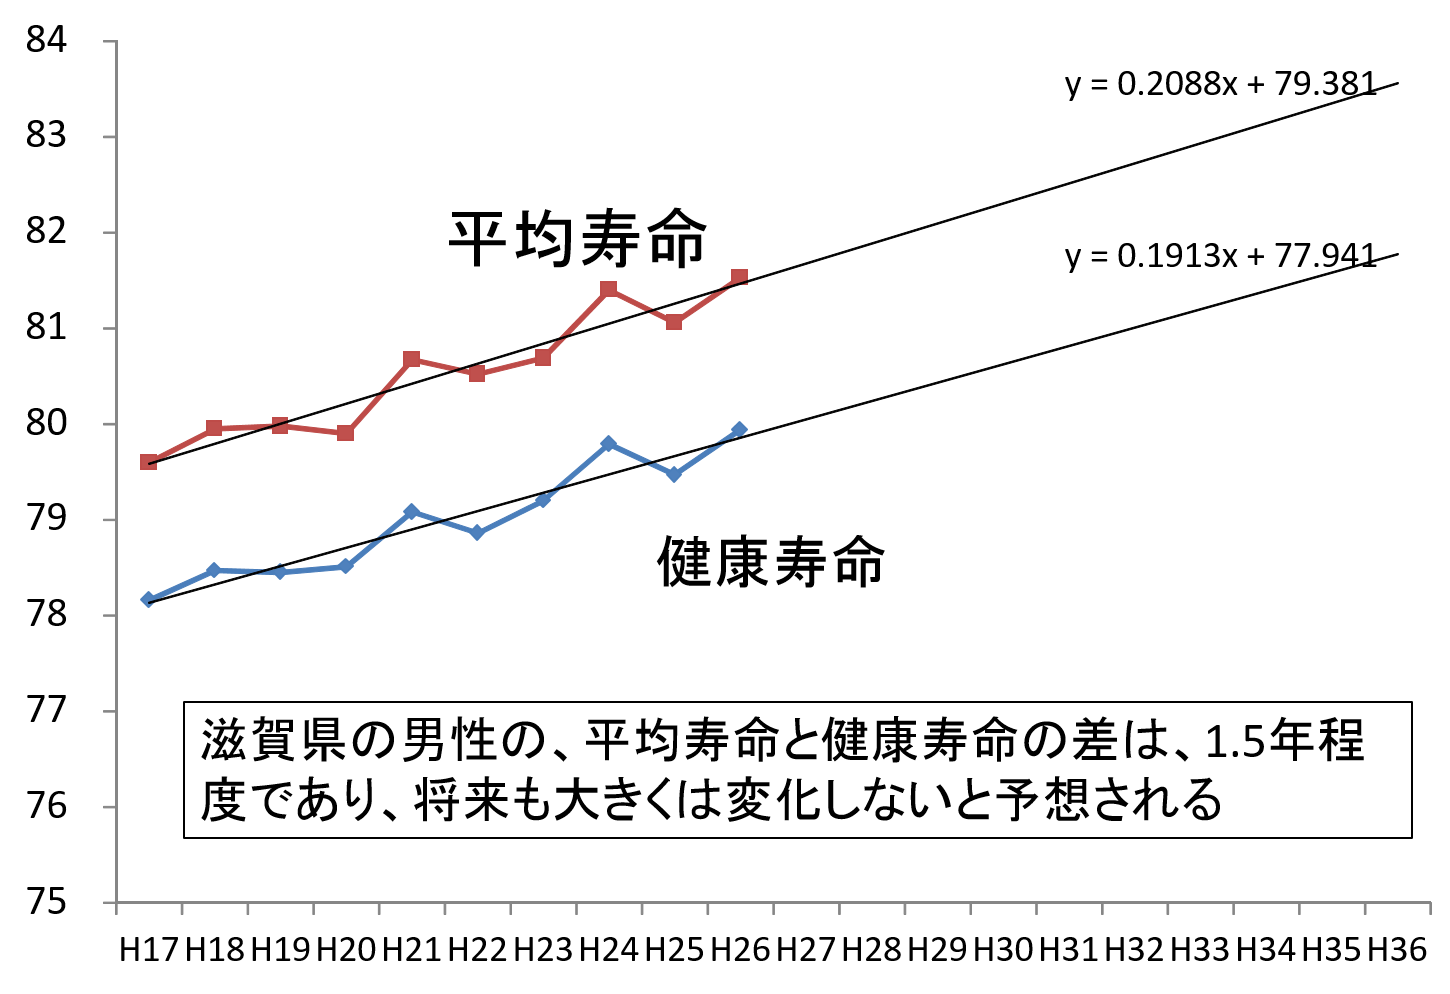
\includegraphics[ width=0.5\linewidth]{fig/fig13.png}
		%     \put(-0.9,0.6){$\leftarrow$滋賀県 男性, 1位}
		%     \put(-0.9,0.25){$\leftarrow$滋賀県 女性, 1位}
		\caption{寿命と健康寿命の予測(男性)}
	\end{center}
\end{figure}

滋賀県の女性の, 平均寿命と健康寿命の差は, 3年程度であるが, 将来その差は拡大すると予想される


\begin{figure}[h!]
	\begin{center}
		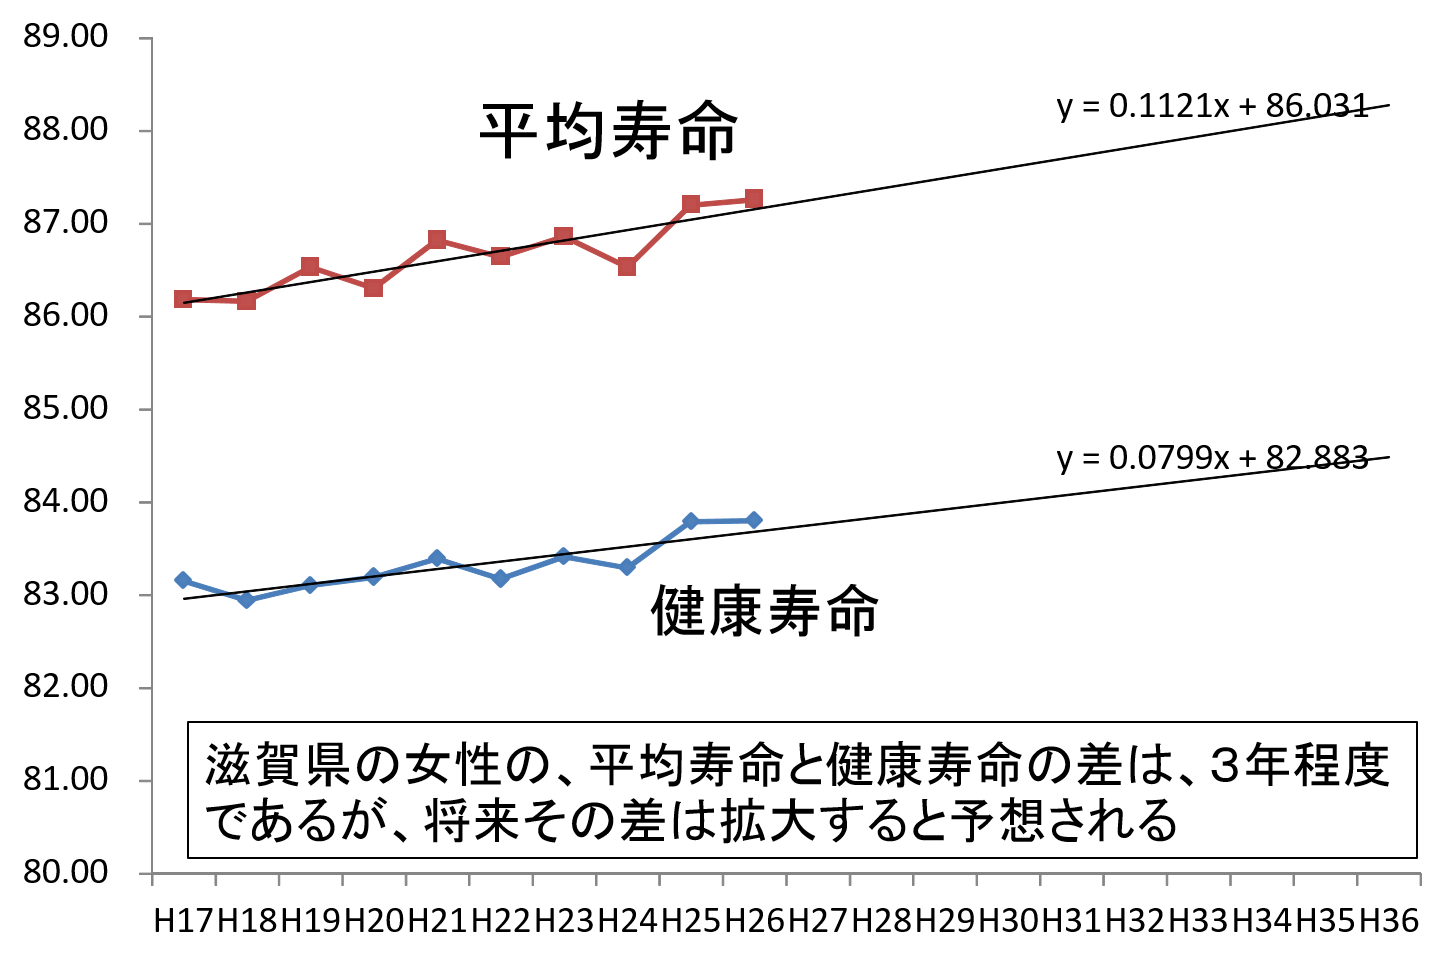
\includegraphics[ width=0.5\linewidth]{fig/fig14.png}
		%     \put(-0.9,0.6){$\leftarrow$滋賀県 男性, 1位}
		%     \put(-0.9,0.25){$\leftarrow$滋賀県 女性, 1位}
		\caption{寿命と健康寿命の予測(女性)}
	\end{center}
\end{figure}

滋賀県は, 男女共, 健康寿命が国より長く, 将来その差は平均寿命の差よりさらに拡大すると予想される


\begin{figure}[h!]
	\begin{center}
		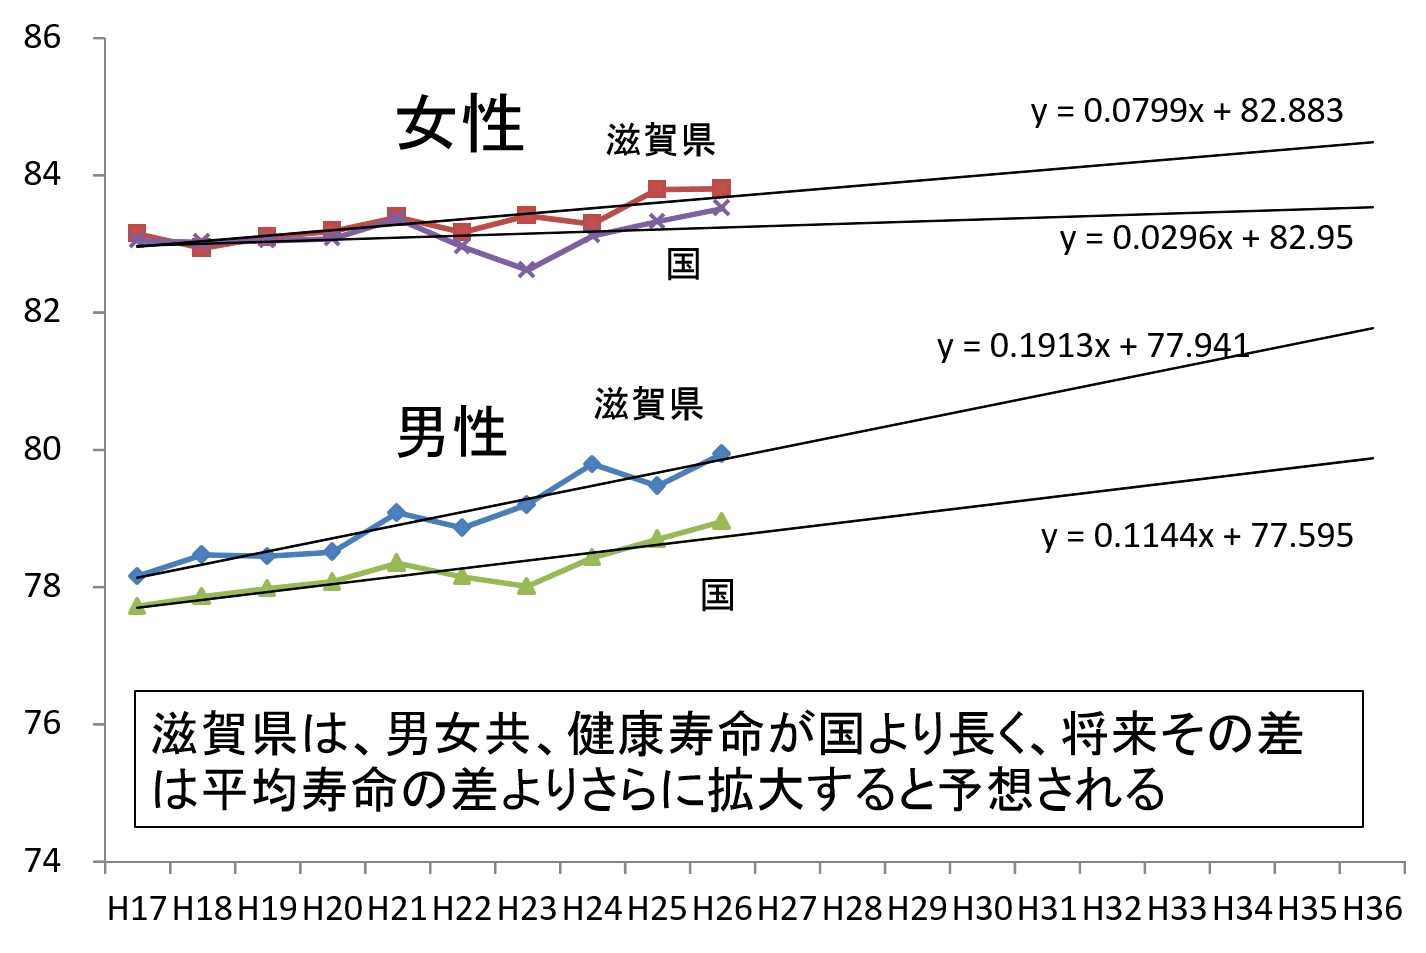
\includegraphics[ width=0.5\linewidth]{fig/fig15.png}
		%     \put(-0.9,0.6){$\leftarrow$滋賀県 男性, 1位}
		%     \put(-0.9,0.25){$\leftarrow$滋賀県 女性, 1位}
		\caption{国, 県の健康寿命の推移と予測}
	\end{center}
\end{figure}



%------------------------------------------------------------
\chapter{参考文献}
%------------------------------------------------------------


%%------------------------------------------------------------
%\chapter{図例}
%%------------------------------------------------------------
%
%
